\section{Performance Analysis}
\label{sec:performance}
To get an overview of the performance of the monitor implementations, each of them was run on at least 100 traces with 10.000 events, which were generated by following specific parameters to show which of these parameters result in faster or slower run times. For this evaluation, the TeSSLa interpreter version 1.2.2 was used and it was run on a computer with an i5-6600k processor running on 4.3 GHz. The operating system was Windows 10.0.19041.0.\\
The run times were measured as the time between the input of all events of one timestamp and the associated output of the TeSSLa interpreter. For that, a program\footnote{This program can be found at \href{https://github.com/HendrikStreichhahn/TeSSLa-Autosar-Timing-Extensions/tree/master/traceGenerator}{https://github.com/HendrikStreichhahn/TeSSLa-Autosar-Timing-Extensions/tree/master/traceGenerator}} was written, which generates traces for each constraint and then measures the time between the input of the events of one timestamp and the output of the TeSSLa interpreter. The communication between the test program and the TeSSLa interpreter is done via the \textit{standard input} and \textit{standard output stream} of the interpreter. The time is measured by the java function \textit{System.nanoTime()} immediately before the events of one timestamp are written into the input stream and immediately after a reaction was received on the output stream. It must be noted that this time measurement is not completely accurate because neither the used java runtime environment nor the operating system was built to fulfill real-time requirements. Therefore, unpredictable delays may occur in the test program, in the java interpreter or between them. However, the averages of the results show what the monitors are capable of and on which input parameters the run time significantly rises.\\
A shortened version of the results will be shown here. The complete results of the runtime measurement can be accessed at Github\footnote{\href{https://github.com/HendrikStreichhahn/TeSSLa-Autosar-Timing-Extensions/tree/master/traceGenerator/results}{https://github.com/HendrikStreichhahn/TeSSLa-Autosar-Timing-Extensions/tree/master/traceGenerator/results}}.

%\footnote{The complete results can be found at  \href{https://github.com/HendrikStreichhahn/TeSSLa-Autosar-Timing-Extensions/tree/master/traceGenerator/results}{https://github.com/HendrikStreichhahn/TeSSLa-Autosar-Timing-Extensions/tree/master/traceGenerator/results}}


\subsubsection{DelayConstraint}
	The \textit{DelayConstraint} was evaluated with 100 Traces of 10.000 events. The traces fulfilled the constraint with the parameters $lower\in\{100, 200, 300, 400, 500, 600, 700, 800,\\ 900, 1000\}$ and $upper=lower$.  The distance of subsequent $source$ event was $2^i$, with $i\in \{0, 1, ..., 10\}$, while the distance between subsequent $source$ events in each trace was smaller than $2*lower$. The shorter the distances between the $source$ event are, the more (at most $upper$, when the distance is 1) events are stored as state.\\
	Figure~\ref{fig:runtimeDelay1} shows the monitor's average run time in dependency of $lower$ and $upper$ for traces with event distances of 1, which means that $upper$ events are stored as the state of the monitor. The run time is nearly constant because the trace generator does not create worst-case scenarios and only one event must be removed from the list at every $target$ event.\\
	Figure~\ref{fig:runtimeDelay2} shows the average run times for this constraint with the parameters $lower=upper=800$ in dependency of the distance of subsequent $source$ events. Two clusters can be observed. The average run times of traces with event distances of $2^0, 2^1,2^2,2^3,2^4,2^5$ are higher than the run times of the other traces. This is because there are timestamps with two events in the first six traces, and in the traces, each timestamp has at most one event. This can be shown by by the following equation. For that:\\
%	\begin{proof}
		Let $lower=upper$ be the distance between $source$ events and their associated $target$ event.\\
		Let $s\in\mathbb{N}_0$ be the first timestamp with a $source$ event in the trace.\\
		Let $dist\in\mathbb{N}$ be the distance between subsequent $source$ events.\\
		The placement of all $source$ events is given by: $s+x*dist$ with $x\in\mathbb N$\\
		The placement of all $target$ events is given by: $s+y*dist + upper$ with $y\in\mathbb N, y<x$\\
		All placements of $source$ and $target$ events, which occur in common timestamps, fulfilled the equation:\\
		\begin{align}
			s+x*dist&=s+y*dist+upper\\
			x*dist&=y*dist+upper\\
			x&= y + \frac{upper}{dist}
		\end{align}
		When $upper=800$, there is no integer solution for $x$ and $y$ for $dist\in{64,128,256,512,1024}$, all events occur in individual timestamps for these distance between $source$ events.\\
		When $dist\in\{1,2,4,8,16,32\}$, there is an integer solution for $x$ and $y$, so there multiple events in individual timestamps.
%	\end{proof}
	\begin{figure}
		\begin{minipage}{0.45\textwidth}
			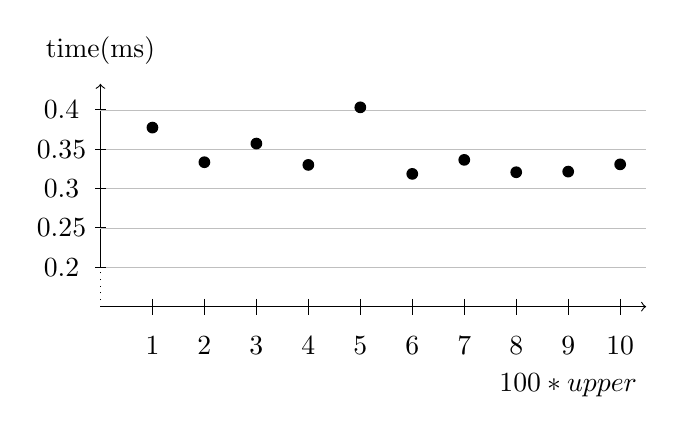
\begin{tikzpicture}[yscale=10, xscale=0.66]
				%time axis
				\draw[->] (0,0.2) -- (0,0.433);
				\draw[dotted](0,0.15)--(0,0.2);
				\node at (0, 0.475){time(ms)};
				
				\foreach \y in {0.2, 0.25, 0.3, 0.35, 0.4}{
					\draw[very thin, lightgray] (0, \y)--(10.5, \y);
					\draw(-0.1, \y)--(0.1, \y);
					\node at (-0.75, \y){\y};
					
				}
				
				\draw[->] (0,0.15) -- (10.5, 0.15);
				\node at (9, 0.05){$100*upper$};
				\foreach \x in {1, 2, ..., 10}{
					\draw(\x, 0.16)--(\x, 0.14);
					\node at (\x, 0.1){${\x}$};
				}
				\node at (1, 0.3774) [circle,fill,inner sep=1.5pt]{};
				\node at (2, 0.3334) [circle,fill,inner sep=1.5pt]{};
				\node at (3, 0.3571) [circle,fill,inner sep=1.5pt]{};
				\node at (4, 0.33) [circle,fill,inner sep=1.5pt]{};
				\node at (5, 0.4031) [circle,fill,inner sep=1.5pt]{};
				\node at (6, 0.3186) [circle,fill,inner sep=1.5pt]{};
				\node at (7, 0.3364) [circle,fill,inner sep=1.5pt]{};
				\node at (8, 0.3207) [circle,fill,inner sep=1.5pt]{};
				\node at (9, 0.3215) [circle,fill,inner sep=1.5pt]{};
				\node at (10, 0.3307) [circle,fill,inner sep=1.5pt]{};
			\end{tikzpicture}
			%\centering
			\caption{Average run times of the \textit{Delay-\\Constraint} with event distances of $2^0=1$}
			\label{fig:runtimeDelay1}
		\end{minipage}\hfill
		\begin{minipage}{0.45\textwidth}
			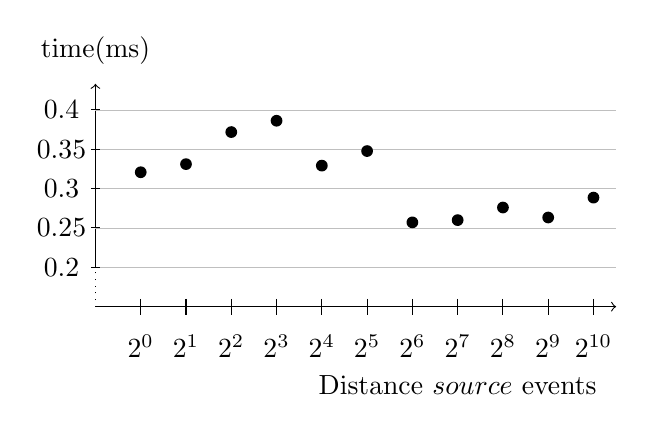
\begin{tikzpicture}[yscale=10, xscale=0.575]
				%time axis
				\draw[->] (0,0.2) -- (0,0.433);
				\draw[dotted](0,0.15)--(0,0.2);
				\node at (0, 0.475){time(ms)};
				
				\foreach \y in {0.2, 0.25, 0.3, 0.35, 0.4}{
					\draw[very thin, lightgray] (0, \y)--(11.5, \y);
					\draw(-0.1, \y)--(0.1, \y);
					\node at (-0.75, \y){\y};
					
				}
				
				\draw[->] (0,0.15) -- (11.5, 0.15);
				\node at (8, 0.05){Distance $source$ events};
				\foreach \x in {0, 1, 2, ..., 10}{
					\draw(\x+1, 0.16)--(\x+1, 0.14);
					\node at (\x+1, 0.1){$2^{\x}$};
				}
				\node at (1, 0.3207) [circle,fill,inner sep=1.5pt]{};
				\node at (2, 0.3310) [circle,fill,inner sep=1.5pt]{};
				\node at (3, 0.3717) [circle,fill,inner sep=1.5pt]{};
				\node at (4, 0.3861) [circle,fill,inner sep=1.5pt]{};
				\node at (5, 0.3291) [circle,fill,inner sep=1.5pt]{};
				\node at (6, 0.3476) [circle,fill,inner sep=1.5pt]{};
				\node at (7, 0.2570) [circle,fill,inner sep=1.5pt]{};
				\node at (8, 0.2599) [circle,fill,inner sep=1.5pt]{};
				\node at (9, 0.2759) [circle,fill,inner sep=1.5pt]{};
				\node at (10, 0.2632) [circle,fill,inner sep=1.5pt]{};
				\node at (11, 0.28846) [circle,fill,inner sep=1.5pt]{};
			\end{tikzpicture}
			\centering
			\caption{Average run times of the \textit{Delay-\\Constraint} with the parameters\\ $lower = upper = 800$}
			\label{fig:runtimeDelay2}
		\end{minipage}
		\centering
	\end{figure}


\subsubsection{StrongDelayConstraint}
	The traces for the evaluation of the \textit{StrongDelayConstraint} were generated with the same parameters as for the previous constraint. Figure~\ref{fig:runtimeStrongDelay1} shows the average run times with a fixed distance between subsequent $source$ events of 1. The results are nearly constant. Figure~\ref{fig:runtimeStrongDelay2} shows the average run times for traces, where $lower$ and $upper$ is fixed at 700 and the distance between subsequent $source$ events is varying. It can be seen that the run times for the traces are separated into two areas, one cluster containing the traces with a $source$ event distance of $2^0, 2^1$ and $2^2$ and one containing the other traces. This clustering has the same reason as in the \textit{DelayConstraint}. It occurs because there are many timestamps with multiple events in some traces and in some traces, all timestamps have at most one event.
	
	%These clusters can be seen at all different values for $lower$ and $upper$, but they are not always containing the traces with the same distance between the $source$ events. The reason for this behaviour is, that in some traces $source$ and $target$ events occur in the same timestamps and in some traces, all timestamps only have at most one timestamp. Because processing two events takes more time than processing one event, the average run time per input timestamp is higher, when more events are processed in less timestamps.\\
%	When the distance between the $source$ events is 1, the parameters $lower$ and $upper$ are set to 700 and 10.000 events are generated, 1.400 timestamps consists of one timestamp and 4.300 timestamp consists of two events. At a distance of 2, 700 timestamps have one event and 4650 timestamps contain 2 events. When the distance is 4, 350 events occur singly and the others occur in 4825 timestamps. In the traces with a $source$ event distance of 8, 16, 32, 64, 128, 256, 512 and 1024, all events occur in individual timestamps, so the run times of them is lower.
%	\begin{proof}
%		Let $lower=upper=700$ be the distance between $source$ events and their associated $target$ event.\\
%		Let $s\in\mathbb{N}_0$ be the first timestamp with an $source$ event in the trace.\\
%		Let $dist\in\mathbb{N}$ be the distance between subsequent $source$ events.\\
%		The placement of all $source$ events is given by: $s+x*dist$ with $x\in\mathbb N$\\
%		The placement of all $target$ events is given by: $s+y*dist + 700$ with $y\in\mathbb N, y<x$\\
%		All placements of $source$ and $target$ events, which occur in common timestamps, fulfilled the equation:\\
%		\begin{align}
%			s+x*dist&=s+y*dist+upper\\
%			x*dist&=y*dist+upper\\
%			x&= y + \frac{upper}{dist}
%		\end{align}
%		Because there is no integer solution for $x$ and $y$ for $dist\in{8,16,32,64,128,256,512,1024}$, all events occur in individual timestamps, when $upper$ is set to 700.
%	\end{proof}
\begin{figure}
	\begin{minipage}{0.45\textwidth}
		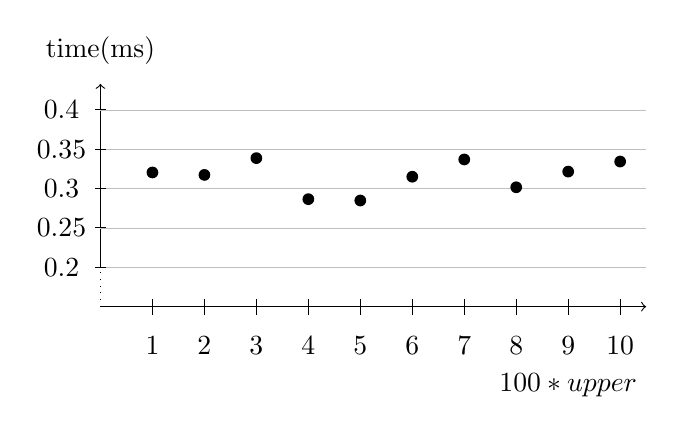
\begin{tikzpicture}[yscale=10, xscale=0.66]
		%time axis
		\draw[->] (0,0.2) -- (0,0.433);
		\draw[dotted](0,0.15)--(0,0.2);
		\node at (0, 0.475){time(ms)};
		
		\foreach \y in {0.2, 0.25, 0.3, 0.35, 0.4}{
			\draw[very thin, lightgray] (0, \y)--(10.5, \y);
			\draw(-0.1, \y)--(0.1, \y);
			\node at (-0.75, \y){\y};
			
		}
		
		\draw[->] (0,0.15) -- (10.5, 0.15);
		\node at (9, 0.05){$100*upper$};
		\foreach \x in {1, 2, ..., 10}{
			\draw(\x, 0.16)--(\x, 0.14);
			\node at (\x, 0.1){${\x}$};
		}
		\node at (1, 0.3204) [circle,fill,inner sep=1.5pt]{};
		\node at (2, 0.3173) [circle,fill,inner sep=1.5pt]{};
		\node at (3, 0.3386) [circle,fill,inner sep=1.5pt]{};
		\node at (4, 0.2865) [circle,fill,inner sep=1.5pt]{};
		\node at (5, 0.2848) [circle,fill,inner sep=1.5pt]{};
		\node at (6, 0.315) [circle,fill,inner sep=1.5pt]{};
		\node at (7, 0.3369) [circle,fill,inner sep=1.5pt]{};
		\node at (8, 0.3016) [circle,fill,inner sep=1.5pt]{};
		\node at (9, 0.3215) [circle,fill,inner sep=1.5pt]{};
		\node at (10, 0.3343) [circle,fill,inner sep=1.5pt]{};
		\end{tikzpicture}
		\centering
		\caption{Average run times of the \textit{Strong-\\DelayConstraint} with event distances of $2^0=1$}
		\label{fig:runtimeStrongDelay1}
	\end{minipage}\hfill
	\begin{minipage}{0.45\textwidth}
		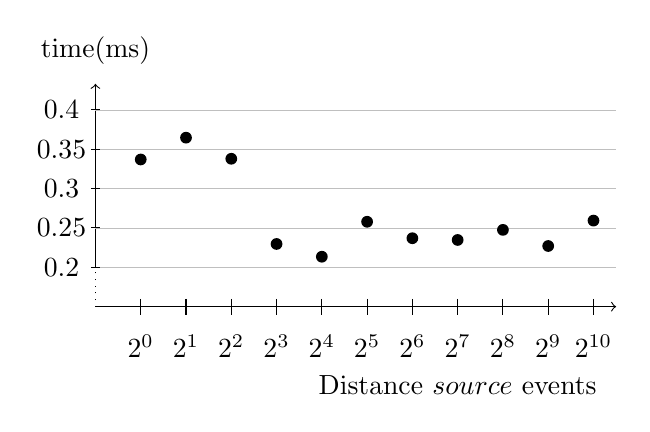
\begin{tikzpicture}[yscale=10, xscale=0.575]
		%time axis
		\draw[->] (0,0.2) -- (0,0.433);
		\draw[dotted](0,0.15)--(0,0.2);
		\node at (0, 0.475){time(ms)};
		
		\foreach \y in {0.2, 0.25, 0.3, 0.35, 0.4}{
			\draw[very thin, lightgray] (0, \y)--(11.5, \y);
			\draw(-0.1, \y)--(0.1, \y);
			\node at (-0.75, \y){\y};
			
		}
		
		\draw[->] (0,0.15) -- (11.5, 0.15);
		\node at (8, 0.05){Distance $source$ events};
		\foreach \x in {0, 1, 2, ..., 10}{
			\draw(\x+1, 0.16)--(\x+1, 0.14);
			\node at (\x+1, 0.1){$2^{\x}$};
		}
		\node at (1, 0.3369) [circle,fill,inner sep=1.5pt]{};
		\node at (2, 0.3646) [circle,fill,inner sep=1.5pt]{};
		\node at (3, 0.3378) [circle,fill,inner sep=1.5pt]{};
		\node at (4, 0.2296) [circle,fill,inner sep=1.5pt]{};
		\node at (5, 0.2134) [circle,fill,inner sep=1.5pt]{};
		\node at (6, 0.2578) [circle,fill,inner sep=1.5pt]{};
		\node at (7, 0.2369) [circle,fill,inner sep=1.5pt]{};
		\node at (8, 0.2347) [circle,fill,inner sep=1.5pt]{};
		\node at (9, 0.2475) [circle,fill,inner sep=1.5pt]{};
		\node at (10, 0.227) [circle,fill,inner sep=1.5pt]{};
		\node at (11, 0.2593) [circle,fill,inner sep=1.5pt]{};
		\end{tikzpicture}
		\centering
		\caption{Average run times of the \textit{StrongDelay-\\Constraint} with the parameters $lower = upper = 700$}
		\label{fig:runtimeStrongDelay2}
	\end{minipage}
\end{figure}




\subsubsection{RepeatConstraint}
	\label{sec_runtimeRepeat}
	The \textit{RepeatConstraint} was evaluated with 100 Traces of 10.000 events. The traces were created with the attributes $span\in\{1,101,201,301\}$, $lower=\{5000,6000,7000,\\8000,9000\}$ and $upper=lower+x$, $x\in\{1000,2000,3000,4000\}$.  Figure~\ref{fig:RepeatConstraintRuntime2} shows the average run time with fixed $span$ and $lower$ parameters and a variable value for $upper$.  Figure~\ref{fig:RepeatConstraintRuntime1} shows the average run times in dependency of the $span$ parameter. As expected by the analysis, the run time was nearly constant and the constraint parameters did not influence the run time.
%	
\begin{figure}
	\centering
	\begin{minipage}{0.45\textwidth}
		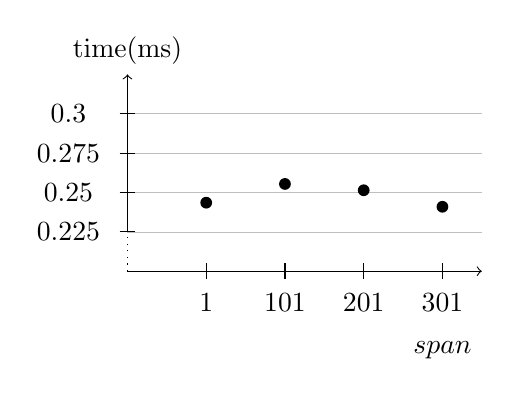
\begin{tikzpicture}[yscale=20]
			%time axis
			\draw[->] (0,0.225) -- (0,0.325);
			\draw[dotted] (0, 0.2) -- (0,0.225);
			\node at (0, 0.34){time(ms)};
			
			\foreach \y in {0.225, 0.25, 0.275, 0.3}{
				\draw[very thin, lightgray] (0, \y)--(4.5, \y);
				\draw(-0.1, \y)--(0.1, \y);
				\node at (-0.75, \y){\y};
				
			}
			
			\draw[->] (0,0.2) -- (4.5, 0.2);
			\node at (4, 0.15){$span$};
			\foreach \x in {0, 1, 2, ..., 3}{
				\draw(\x+1, 0.205)--(\x+1, 0.195);
			}
			\node at (1, 0.18){$1$};
			\node at (2, 0.18){$101$};
			\node at (3, 0.18){$201$};
			\node at (4, 0.18){$301$};
			
			%\draw (1, 0.2491) -- (2, 0.2743) -- (3, 0.25835) -- (4, 0.2737);
			
			\node at (1, 0.2435) [circle,fill,inner sep=1.5pt]{};
			\node at (2, 0.2554) [circle,fill,inner sep=1.5pt]{};
			\node at (3, 0.2514) [circle,fill,inner sep=1.5pt]{};
			\node at (4, 0.2409) [circle,fill,inner sep=1.5pt]{};
		\end{tikzpicture}
		\centering
		\caption{Average run times of the\\ \textit{RepeatConstraint} with the\\ parameters $lower = 6000, upper = 9000$}
		\label{fig:RepeatConstraintRuntime1}
	\end{minipage}\hfill
	\begin{minipage}{0.45\textwidth}
		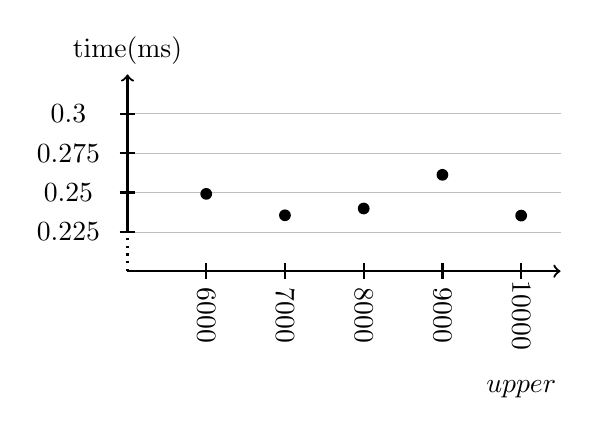
\begin{tikzpicture}[thick, yscale=20]
			%time axis
			\draw[->] (0,0.225) -- (0,0.325);
			\draw[dotted] (0, 0.2) -- (0,0.225);
			\node at (0, 0.34){time(ms)};
			
			\foreach \y in {0.225, 0.25, 0.275, 0.3}{
				\draw[very thin, lightgray] (0, \y)--(5.5, \y);
				\draw(-0.1, \y)--(0.1, \y);
				\node at (-0.75, \y){\y};
				
			}
			
			\draw[->] (0,0.2) -- (5.5, 0.2);
			\node at (5, 0.125){$upper$};
			\foreach \x in {0, 1, 2, ..., 4}{
				\draw(\x+1, 0.205)--(\x+1, 0.195);
			}
			\node[rotate=270] at (1, 0.172){$6000$};
			\node[rotate=270] at (2, 0.172){$7000$};
			\node[rotate=270] at (3, 0.172){$8000$};
			\node[rotate=270] at (4, 0.172){$9000$};		
			\node[rotate=270] at (5, 0.172){$10000$};
			\node at (1, 0.2491) [circle,fill,inner sep=1.5pt]{};
			\node at (2, 0.2355) [circle,fill,inner sep=1.5pt]{};
			\node at (3, 0.2398) [circle,fill,inner sep=1.5pt]{};
			\node at (4, 0.2612) [circle,fill,inner sep=1.5pt]{};
			\node at (5, 0.2353) [circle,fill,inner sep=1.5pt]{};
		\end{tikzpicture}
		\centering
		\caption{Average run times of the\\ \textit{RepeatConstraint} with the parameters\\ $lower = 5000, span = 1$}
		\label{fig:RepeatConstraintRuntime2}
	\end{minipage}
\end{figure}
%
%\begin{figure}
%	\begin{tikzpicture}[thick, yscale=20]
%	%time axis
%	\draw[->] (0,0.225) -- (0,0.3);
%	\draw[dotted] (0, 0.2) -- (0,0.225);
%	\node at (0, 0.325){time(ms)};
%	
%	\foreach \y in {0.225, 0.25, 0.275}{
%		\draw[very thin, lightgray] (0, \y)--(5.5, \y);
%		\draw(-0.1, \y)--(0.1, \y);
%		\node at (-0.75, \y){\y};
%		
%	}
%	
%	\draw[->] (0,0.2) -- (5.5, 0.2);
%	\node at (5, 0.16){$upper$};
%	\foreach \x in {0, 1, 2, ..., 4}{
%		\draw(\x+1, 0.205)--(\x+1, 0.195);
%		%\node at (\x+1, -0.05){$2^{\x}$};
%	}
%	\node at (1, 0.18){$6000$};
%	\node at (2, 0.18){$7000$};
%	\node at (3, 0.18){$8000$};
%	\node at (4, 0.18){$9000$};
%	\node at (5, 0.18){$10000$};
%	
%	
%	\node at (1, 0.2491) [circle,fill,inner sep=1.5pt]{};
%	\node at (2, 0.2348) [circle,fill,inner sep=1.5pt]{};
%	\node at (3, 0.2269) [circle,fill,inner sep=1.5pt]{};
%	\node at (4, 0.2334) [circle,fill,inner sep=1.5pt]{};
%	\node at (5, 0.2404) [circle,fill,inner sep=1.5pt]{};
%	\end{tikzpicture}
%	\centering
%	\caption{Average run times of the \textit{RepeatConstraint} with the parameters $span = 1,  lower = 5000$}
%	\label{fig:RepeatConstraintRuntime3}
%\end{figure}

\subsubsection{RepetitionConstraint}
	The traces for this constraint were created with the parameters $span\in\{1,100,250,500\}$, $lower=\{500,600,700,800,900\}$ $upper=lower+x$, $x\in{400,500,600,700,800}$ and $jitter=\frac{lower}{2}$.\\
	Figure~\ref{fig:RepetitionConstraintRuntime1} and \ref{fig:RepetitionConstraintRuntime2} show the average run times of the monitor with the parameters $lower=500$(700) and $upper=900$(1100) with different values of the $span$ parameter. Figure~\ref{fig:RepetitionConstraintRuntime3} shows the average run time in dependency on the $upper$ parameter. As expected in the analysis, the parameters did not influence the run times and the run times are nearly constant.
\begin{figure}
	\centering
	\begin{minipage}{0.45\textwidth}
		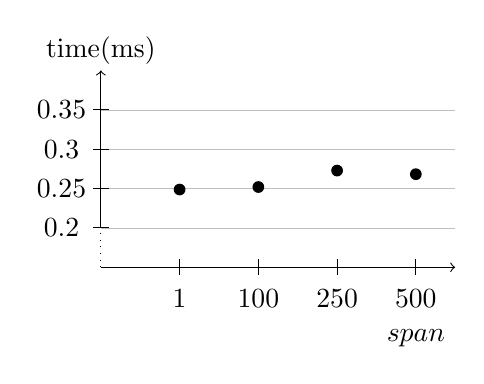
\begin{tikzpicture}[yscale=10]
		%time axis
		\draw[->] (0,0.2) -- (0,0.4);
		\draw[dotted] (0, 0.15) -- (0,0.2);
		\node at (0, 0.425){time(ms)};
			
		\foreach \y in {0.2, 0.25, 0.3, 0.35}{
			\draw[very thin, lightgray] (0, \y)--(4.5, \y);
			\draw(-0.1, \y)--(0.1, \y);
			\node at (-0.5, \y){\y};
		
		}
		
		\draw[->] (0,0.15) -- (4.5, 0.15);
		\node at (4, 0.06){$span$};
		\foreach \x in {0, 1, 2, ..., 3}{
			\draw(\x+1, 0.16)--(\x+1, 0.14);
		}
		\node at (1, 0.11){$1$};
		\node at (2, 0.11){$100$};
		\node at (3, 0.11){$250$};
		\node at (4, 0.11){$500$};
		\node at (1, 0.2487) [circle,fill,inner sep=1.5pt]{};
		\node at (2, 0.2519) [circle,fill,inner sep=1.5pt]{};
		\node at (3, 0.2728) [circle,fill,inner sep=1.5pt]{};
		\node at (4, 0.2682) [circle,fill,inner sep=1.5pt]{};
		\end{tikzpicture}
		\centering
		\caption{Average run times of the\\ \textit{RepetitionConstraint} with the\\ parameters $lower = 500, upper = 900$}
		\label{fig:RepetitionConstraintRuntime1}
	\end{minipage}\hfill
	\begin{minipage}{0.45\textwidth}
		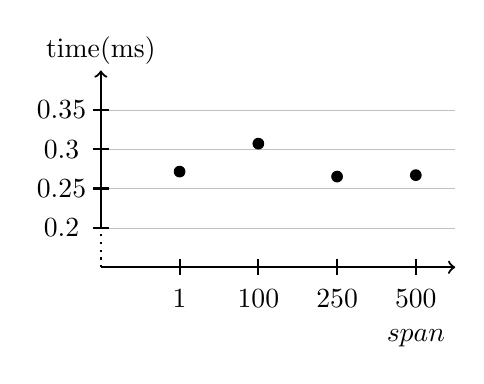
\begin{tikzpicture}[thick, yscale=10]
		%time axis
		\draw[->] (0,0.2) -- (0,0.4);
		\draw[dotted] (0, 0.15) -- (0,0.2);
		\node at (0, 0.425){time(ms)};
		
		\foreach \y in {0.2, 0.25, 0.3, 0.35}{
			\draw[very thin, lightgray] (0, \y)--(4.5, \y);
			\draw(-0.1, \y)--(0.1, \y);
			\node at (-0.5, \y){\y};
		
		}
		
		\draw[->] (0,0.15) -- (4.5, 0.15);
		\node at (4, 0.06){$span$};
		\foreach \x in {0, 1, 2, ..., 3}{
			\draw(\x+1, 0.16)--(\x+1, 0.14);
		}
		\node at (1, 0.11){$1$};
		\node at (2, 0.11){$100$};
		\node at (3, 0.11){$250$};
		\node at (4, 0.11){$500$};
		\node at (1, 0.2715) [circle,fill,inner sep=1.5pt]{};
		\node at (2, 0.307) [circle,fill,inner sep=1.5pt]{};
		\node at (3, 0.2652) [circle,fill,inner sep=1.5pt]{};
		\node at (4, 0.267) [circle,fill,inner sep=1.5pt]{};
		\end{tikzpicture}
		\centering
		\caption{Average run times of the\\ \textit{RepetitionConstraint} with the parameters\\ $lower = 600, upper = 1000$}
		\label{fig:RepetitionConstraintRuntime2}
	\end{minipage}
\end{figure}
	
\begin{figure}
	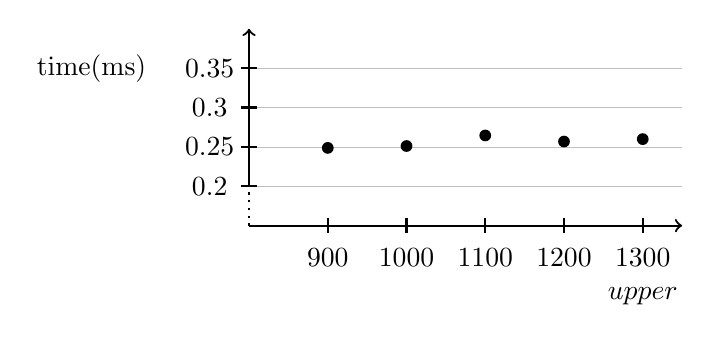
\begin{tikzpicture}[thick, yscale=10]
	%time axis
	\draw[->] (0,0.2) -- (0,0.4);
	\draw[dotted] (0, 0.15) -- (0,0.2);
	\node at (-2, 0.35){time(ms)};
	
	\foreach \y in {0.2, 0.25, 0.3, 0.35}{
		\draw[very thin, lightgray] (0, \y)--(5.5, \y);
		\draw(-0.1, \y)--(0.1, \y);
		\node at (-0.5, \y){\y};
		
	}
	
	\draw[->] (0,0.15) -- (5.5, 0.15);
	\node at (5, 0.06){$upper$};
	\foreach \x in {0, 1, 2, ..., 4}{
		\draw(\x+1, 0.16)--(\x+1, 0.14);
		%\node at (\x+1, -0.05){$2^{\x}$};
	}
	\node at (1, 0.11){$900$};
	\node at (2, 0.11){$1000$};
	\node at (3, 0.11){$1100$};
	\node at (4, 0.11){$1200$};
	\node at (5, 0.11){$1300$};
	
	
	\node at (1, 0.2487) [circle,fill,inner sep=1.5pt]{};
	\node at (2, 0.2511) [circle,fill,inner sep=1.5pt]{};
	\node at (3, 0.2645) [circle,fill,inner sep=1.5pt]{};
	\node at (4, 0.2568) [circle,fill,inner sep=1.5pt]{};
	\node at (5, 0.2599) [circle,fill,inner sep=1.5pt]{};
	\end{tikzpicture}
	\centering
	\caption{Average run times of the \textit{RepetitionConstraint} with the parameters $span = 1,  lower = 500$}
	\label{fig:RepetitionConstraintRuntime3}
\end{figure}
	
	
\subsubsection{SynchronizationConstraint}
The traces for the time measurement were created with two to five event streams, $tolerance$ values from 1 to 155 and distances between subsequent synchronization clusters from 1 to 200.\\
Figure~\ref{fig:SynchronizationConstraintConstraintRunTime1} shows the average run times of the \textit{SynchronizationConstraint} monitor, which was checking traces with three event streams. The synchronization clusters were 200 timestamps apart, so they did not overlap and in each cluster, $\lfloor \frac{tolerance}{2}\rfloor$ events occurred.\\
Figure~\ref{fig:SynchronizationConstraintConstraintRunTime2} shows the average run times of the monitor with traces of three streams, a $tolerance$ value of 91 and a distance between clusters of 182. So again, the clusters were not overlapping. It can be seen that the run times grow linear when increasing the number of events in each cluster. This matches the expectation because the more events occur in an interval of the length $tolerance$, the more events need to be stored and considered in each input timestamp.
\begin{figure}
	\centering
	\begin{minipage}{0.45\textwidth}
		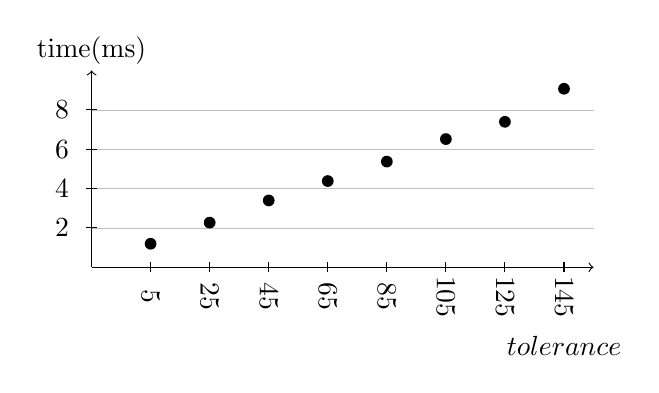
\begin{tikzpicture}[yscale=0.25, xscale=1.5]
		%time axis
		\draw[->] (0,0) -- (0,10);
		\node at (0, 11){time(ms)};
		
		\foreach \y in {2, 4, 6, 8}{
			\draw[very thin, lightgray] (0, \y)--(4.25, \y);
			\draw(-0.05, \y)--(0.05, \y);
			\node at (-0.25, \y){\y};
			
		}
		
		\draw[->] (0,0) -- (4.25, 0);
		\node at (4, -4){$tolerance$};
		\foreach \x in {0.5, 1, 1.5, 2, 2.5, 3, 3.5, 4}{
			\draw(\x, 0.25)--(\x, -0.25);
		}
		\node[rotate=270] at (0.5, -1.5){$5$};
		\node[rotate=270] at (1, -1.5){$25$};
		\node[rotate=270] at (1.5, -1.5){$45$};
		\node[rotate=270] at (2, -1.5){$65$};
		\node[rotate=270] at (2.5, -1.5){$85$};
		\node[rotate=270] at (3, -1.5){$105$};
		\node[rotate=270] at (3.5, -1.5){$125$};
		\node[rotate=270] at (4, -1.5){$145$};
		\node at (0.5, 1.1945) [circle,fill,inner sep=1.5pt]{};
		\node at (1, 2.2673) [circle,fill,inner sep=1.5pt]{};
		\node at (1.5, 3.3946) [circle,fill,inner sep=1.5pt]{};
		\node at (2, 4.3806) [circle,fill,inner sep=1.5pt]{};
		\node at (2.5, 5.3684) [circle,fill,inner sep=1.5pt]{};
		\node at (3,  6.5125) [circle,fill,inner sep=1.5pt]{};
		\node at (3.5, 7.3889) [circle,fill,inner sep=1.5pt]{};
		\node at (4, 9.0679) [circle,fill,inner sep=1.5pt]{};
		\end{tikzpicture}
		\centering
		\caption{Average run times of the\\ \textit{SynchronizationConstraint} with three event\\ streams, $\lfloor\frac{tolerance}{2}\rfloor$ events per cluster and stream\\ and a cluster distance of 200}
		\label{fig:SynchronizationConstraintConstraintRunTime1}
	\end{minipage}\hfill
	\begin{minipage}{0.45\textwidth}
		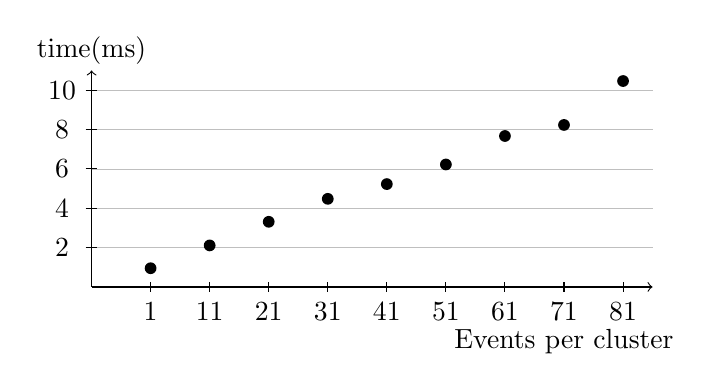
\begin{tikzpicture}[yscale=0.25, xscale=1.5]
			%time axis
			\draw[->] (0,0) -- (0,11);
			\node at (0, 12){time(ms)};
			
			\foreach \y in {2, 4, ..., 10}{
				\draw[very thin, lightgray] (0, \y)--(4.75, \y);
				\draw(-0.05, \y)--(0.05, \y);
				\node at (-0.25, \y){\y};
				
			}
			
			\draw[->] (0,0) -- (4.75,0);
			\node at (4, -2.75){Events per cluster};
			\foreach \x in {0.5, 1, 1.5, 2, 2.5, 3, 3.5, 4, 4.5}{
				\draw(\x, 0.25)--(\x, -0.25);
			}
			\node at (0.5, -1.25){$1$};
			\node at (1, -1.25){$11$};
			\node at (1.5, -1.25){$21$};
			\node at (2, -1.25){$31$};
			\node at (2.5, -1.25){$41$};
			\node at (3, -1.25){$51$};
			\node at (3.5, -1.25){$61$};
			\node at (4, -1.25){$71$};
			\node at (4.5, -1.25){$81$};
			\node at (0.5, 0.9513) [circle,fill,inner sep=1.5pt]{};
			\node at (1, 2.1098) [circle,fill,inner sep=1.5pt]{};
			\node at (1.5, 3.3105) [circle,fill,inner sep=1.5pt]{};
			\node at (2, 4.4764) [circle,fill,inner sep=1.5pt]{};
			\node at (2.5, 5.2265) [circle,fill,inner sep=1.5pt]{};
			\node at (3, 6.22116) [circle,fill,inner sep=1.5pt]{};
			\node at (3.5, 7.6682) [circle,fill,inner sep=1.5pt]{};
			\node at (4, 8.2293) [circle,fill,inner sep=1.5pt]{};
			\node at (4.5, 10.461) [circle,fill,inner sep=1.5pt]{};
		\end{tikzpicture}
		\centering
		\caption{Average run times of the\\ \textit{SynchronizationConstraint} with three event streams,\\ $tolerance=91$ and a cluster distance of $182$ }
		\label{fig:SynchronizationConstraintConstraintRunTime2}
	\end{minipage}
\end{figure}


\subsubsection{StrongSynchronizationConstraint}
	The \textit{StrongSynchronizationConstraint} monitor was evaluated on traces generated with $tolerance$ values from 1 to 100, distances between synchronization clusters from 2 to 246 and two to five event streams.\\
	Figure~\ref{fig:StrongSynchronizationConstraintConstraintRunTime1} shows the average run time of the monitor with the parameters $tolerance = 37$ and a cluster distance of 2 so that 19 clusters are overlapping. It can be seen that the run time increases when more input streams are used. This behavior was expected because the more input streams are considered, the more events need to be processed and the larger is the information about synchronization clusters, which are stored in the monitor.\\
	In Figure~\ref{fig:StrongSynchronizationConstraintConstraintRunTime2}, a fixed number of input streams was used and the cluster distance was 128. The run time was nearly constant because the synchronization clusters did not overlap and therefore, only one cluster must be considered in each timestamp. The runtime at $tolerance=1$ is slightly larger because events occur more often together in one timestamp. The linear growth, as described in the analysis, is only reached in worst-cases, where the events do not occur in clusters.
\begin{figure}
	\centering
	\begin{minipage}{0.45\textwidth}
%		\begin{tikzpicture}[yscale=20]
%		%time axis
%		\draw[->] (0,0.775) -- (0,0.875);
%		\draw[dotted] (0, 0.75) -- (0,0.775);
%		\node at (0, 0.9){time(ms)};
%		
%		\foreach \y in {0.775, 0.8, 0.825, 0.85}{
%			\draw[very thin, lightgray] (0, \y)--(4.5, \y);
%			\draw(-0.1, \y)--(0.1, \y);
%			\node at (-1, \y){\y};
%			
%		}
%		
%		\draw[->] (0,0.75) -- (4.5, 0.75);
%		\node at (3, 0.7){Cluster Distance};
%		\foreach \x in { 1, 2, 3, 4}{
%			\draw(\x, 0.745)--(\x, 0.755);
%		}
%		\node[rotate=270] at (1, 0.7255){$2$};
%		\node[rotate=270] at (2, 0.7255){$8$};
%		\node[rotate=270] at (3, 0.7255){$32$};
%		\node[rotate=270] at (4, 0.7255){$128$};
%		\node at (1, 0.7828) [circle,fill,inner sep=1.5pt]{};
%		\node at (2, 0.8206) [circle,fill,inner sep=1.5pt]{};
%		\node at (3, 0.7894) [circle,fill,inner sep=1.5pt]{};
%		\node at (4, 0.8319) [circle,fill,inner sep=1.5pt]{};
%		\end{tikzpicture}
%		\centering
%		\caption{Average run times of the\\ \textit{StrongSynchronizationConstraint} with two\\ event streams and $tolerance=1$}
%		\label{fig:StrongSynchronizationConstraintConstraintRunTime1}
		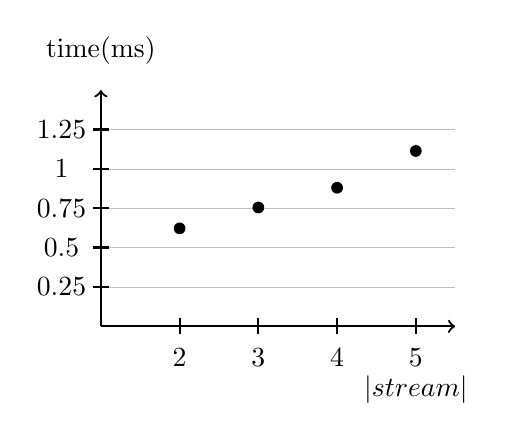
\begin{tikzpicture}[thick, yscale=2]
		%time axis
		\draw[->] (0,0) -- (0, 1.5);
		\node at (0, 1.75){time(ms)};
		
		\foreach \y in {0.25, 0.5, 0.75, 1, 1.25}{
			\draw[very thin, lightgray] (0, \y)--(4.5, \y);
			\draw(-0.1, \y)--(0.1, \y);
			\node at (-0.5, \y){\y};
			
		}
		
		\draw[->] (0,0) -- (4.5, 0);
		\node at (4, -0.4){$|stream|$};
		\foreach \x in {1,2,3,4}{
			\draw(\x, 0.05)--(\x, -0.05);
		}
		\node at (1, -0.2){$2$};
		\node at (2, -0.2){$3$};
		\node at (3, -0.2){$4$};
		\node at (4, -0.2){$5$};
		\node at (1, 0.6221) [circle,fill,inner sep=1.5pt]{};
		\node at (2, 0.7546) [circle,fill,inner sep=1.5pt]{};
		\node at (3, 0.8799) [circle,fill,inner sep=1.5pt]{};
		\node at (4, 1.1135) [circle,fill,inner sep=1.5pt]{};
		\end{tikzpicture}
		\centering
		\caption{Average run times of the\\ \textit{StrongSynchronizationConstraint} with\\$tolerance=37$ and a cluster distance of 2}
		\label{fig:StrongSynchronizationConstraintConstraintRunTime1}
	\end{minipage}\hfill
	\begin{minipage}{0.45\textwidth}
		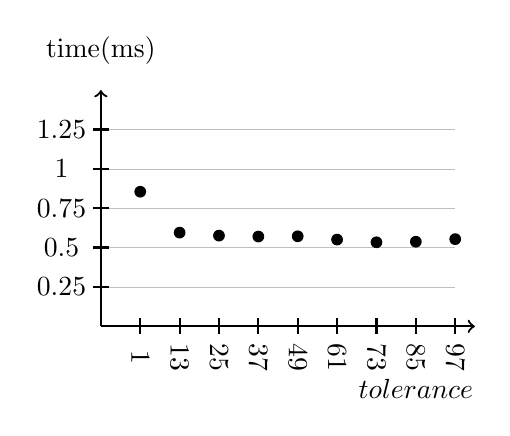
\begin{tikzpicture}[thick, yscale=2]
		%time axis
		\draw[->] (0,0) -- (0, 1.5);
		\node at (0, 1.75){time(ms)};
		
		\foreach \y in {0.25, 0.5, 0.75, 1, 1.25}{
			\draw[very thin, lightgray] (0, \y)--(4.5, \y);
			\draw(-0.1, \y)--(0.1, \y);
			\node at (-0.5, \y){\y};
			
		}
		
		\draw[->] (0,0) -- (4.75, 0);
		\node at (4, -0.4){$tolerance$};
		\foreach \x in {0.5, 1, ..., 4.5}{
			\draw(\x, 0.05)--(\x, -0.05);
		}
		\node[rotate=270] at (0.5, -0.2){$1$};
		\node[rotate=270] at (1, -0.2){$13$};
		\node[rotate=270] at (1.5, -0.2){$25$};
		\node[rotate=270] at (2, -0.2){$37$};
		\node[rotate=270] at (2.5, -0.2){$49$};
		\node[rotate=270] at (3, -0.2){$61$};
		\node[rotate=270] at (3.5, -0.2){$73$};
		\node[rotate=270] at (4, -0.2){$85$};
		\node[rotate=270] at (4.5, -0.2){$97$};
		\node at (0.5, 0.8547) [circle,fill,inner sep=1.5pt]{};
		\node at (1, 0.595) [circle,fill,inner sep=1.5pt]{};
		\node at (1.5, 0.5761) [circle,fill,inner sep=1.5pt]{};
		\node at (2, 0.5701) [circle,fill,inner sep=1.5pt]{};
		\node at (2.5, 0.5718) [circle,fill,inner sep=1.5pt]{};
		\node at (3, 0.5507) [circle,fill,inner sep=1.5pt]{};
		\node at (3.5, 0.5336) [circle,fill,inner sep=1.5pt]{};
		\node at (4, 0.5372) [circle,fill,inner sep=1.5pt]{};
		\node at (4.5, 0.5537) [circle,fill,inner sep=1.5pt]{};
		\end{tikzpicture}
		\centering
		\caption{Average run times of the\\ \textit{StrongSynchronizationConstraint} with four\\ event streams and a cluster distance of 128}
		\label{fig:StrongSynchronizationConstraintConstraintRunTime2}
	\end{minipage}
\end{figure}




\subsubsection{ExecutionTimeConstraint}
	The run time evaluation of the \textit{ExecutionTimeConstraint} monitor was done by traces, which fulfill the constraint the parameters $lower\in\{100,300,500,700,900\}$ and $upper=lower+x$, $x\in\{100,600,1100,1600,2100\}$. For each combination of these parameters, one trace with 1, 11, 21 and 31 preemptions between the $start$ and $end$ event were created. In figure~\ref{fig:ExecutionTimeConstraintRunTime1}, the average run time with fixed $lower$ and $upper$ can be seen. In figure~\ref{fig:ExecutionTimeConstraintRunTime2}, $lower$ and the number of preemptions is fixed. A correlation between the input parameters and the run times can not be observed, which was expected, because the run time is independent of the parameters or the placement of events, like stated in chapter~\ref{chapter-implementation}.
\begin{figure}
	\centering
	\begin{minipage}{0.45\textwidth}
		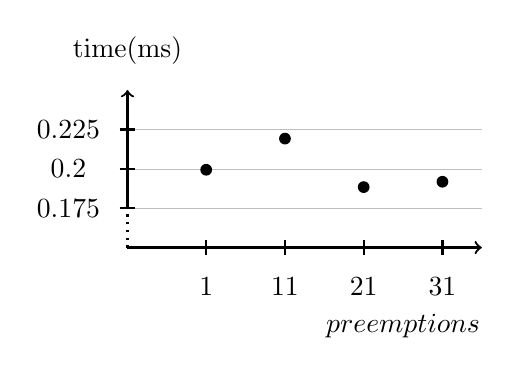
\begin{tikzpicture}[thick, yscale=20]
			%time axis
			\draw[->] (0,0.175) -- (0,0.25);
			\draw[dotted] (0, 0.15) -- (0,0.175);
			\node at (0, 0.275){time(ms)};
			
			\foreach \y in {0.175, 0.2, 0.225}{
				\draw[very thin, lightgray] (0, \y)--(4.5, \y);
				\draw(-0.1, \y)--(0.1, \y);
				\node at (-0.75, \y){\y};
				
			}
			
			\draw[->] (0,0.15) -- (4.5, 0.15);
			\node at (3.5, 0.1){$preemptions$};
			\foreach \x in {0, 1, 2, ..., 3}{
				\draw(\x+1, 0.145)--(\x+1, 0.155);
			}
			\node at (1, 0.125){$1$};
			\node at (2, 0.125){$11$};
			\node at (3, 0.125){$21$};
			\node at (4, 0.125){$31$};
			\node at (1, 0.1994) [circle,fill,inner sep=1.5pt]{};
			\node at (2, 0.2192) [circle,fill,inner sep=1.5pt]{};
			\node at (3, 0.1884) [circle,fill,inner sep=1.5pt]{};
			\node at (4, 0.1918) [circle,fill,inner sep=1.5pt]{};
		\end{tikzpicture}
		\centering
		\caption{Average run times of the\\ \textit{ExecutionTimeConstraint} with the\\ parameters $lower = 100, upper = 1700$}
		\label{fig:ExecutionTimeConstraintRunTime1}
	\end{minipage}\hfill
	\begin{minipage}{0.45\textwidth}
		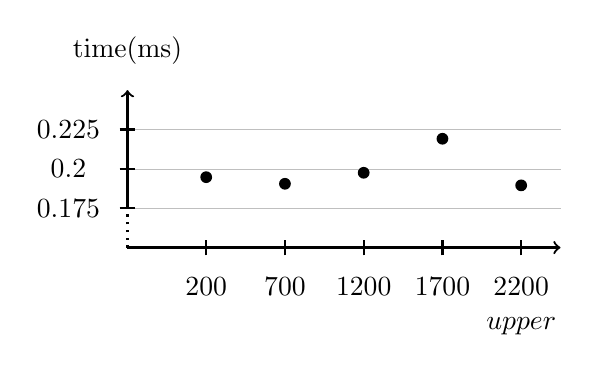
\begin{tikzpicture}[thick, yscale=20]
			%time axis
			\draw[->] (0,0.175) -- (0,0.25);
			\draw[dotted] (0, 0.15) -- (0,0.175);
			\node at (0, 0.275){time(ms)};
			
			\foreach \y in {0.175, 0.2, 0.225}{
				\draw[very thin, lightgray] (0, \y)--(5.5, \y);
				\draw(-0.1, \y)--(0.1, \y);
				\node at (-0.75, \y){\y};
				
			}
			
			\draw[->] (0,0.15) -- (5.5, 0.15);
			\node at (5, 0.1){$upper$};
			\foreach \x in {0, 1, 2, ..., 3, 4}{
				\draw(\x+1, 0.145)--(\x+1, 0.155);
			}
			\node at (1, 0.125){$200$};
			\node at (2, 0.125){$700$};
			\node at (3, 0.125){$1200$};
			\node at (4, 0.125){$1700$};
			\node at (5, 0.125){$2200$};
			\node at (1, 0.1947) [circle,fill,inner sep=1.5pt]{};
			\node at (2, 0.1905) [circle,fill,inner sep=1.5pt]{};
			\node at (3, 0.1975) [circle,fill,inner sep=1.5pt]{};
			\node at (4, 0.2191) [circle,fill,inner sep=1.5pt]{};
			\node at (5, 0.1895) [circle,fill,inner sep=1.5pt]{};
		\end{tikzpicture}
		\centering
		\caption{Average run times of the\\ \textit{ExecutionTimeConstraint} with the parameters\\ $lower = 100, preemptions = 11$}
		\label{fig:ExecutionTimeConstraintRunTime2}
	\end{minipage}
\end{figure}

\subsubsection{OrderConstraint}
The \textit{OrderConstraint} monitor was evaluated on traces with distances between subsequent $source$ events between 1 and 91 in steps of 10 and maximal distances between the $i^{th}$ $source$ and $target$ event between 0 and 45 in steps of 5. In traces, where the distance between the $source$ events and their associated $target$ events was 0, or the distance between subsequent $source$ events was 1, the run time was significantly larger as in the other traces. The reason for this is that the smaller the distance between the $source$ and $target$ events are, the more often two events occur in the same timestamp, which means that two events must be processed in one timestamp instead of one, which requires more time.
\begin{figure}
	\begin{minipage}{0.45\textwidth}
		\centering
		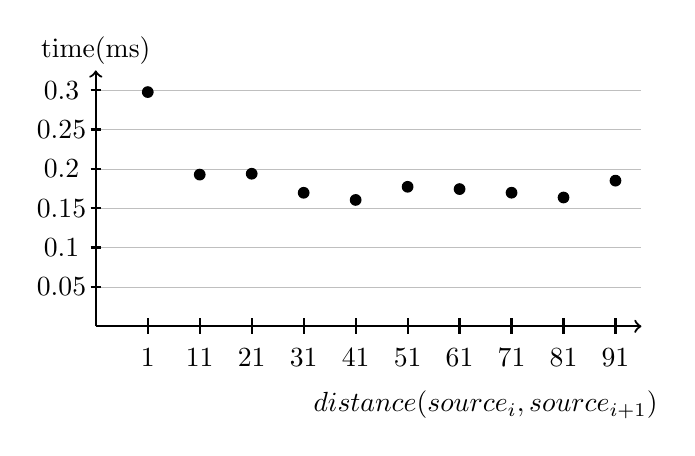
\begin{tikzpicture}[thick, yscale=10, xscale=0.66]
		%time axis
		\draw[->] (0,0) -- (0,0.325);
		\node at (0, 0.35){time(ms)};
		
		\foreach \y in {0.05, 0.1, 0.15, 0.2, 0.25, 0.3}{
			\draw[very thin, lightgray] (0, \y)--(10.5, \y);
			\draw(-0.1, \y)--(0.1, \y);
			\node at (-0.66, \y){\y};
			
		}
		
		\draw[->] (0,0) -- (10.5, 0);
		\node at (7.5, -0.1){$distance(source_i, source_{i+1})$};
		\foreach \x in {0, 1, 2, ..., 9}{
			\draw(\x+1, 0.01)--(\x+1, -0.01);
		}
		\node at (1, -0.04){$1$};
		\node at (2, -0.04){$11$};
		\node at (3, -0.04){$21$};
		\node at (4, -0.04){$31$};
		\node at (5, -0.04){$41$};
		\node at (6, -0.04){$51$};
		\node at (7, -0.04){$61$};
		\node at (8, -0.04){$71$};
		\node at (9, -0.04){$81$};
		\node at (10, -0.04){$91$};
		
		\node at (1, 0.2975) [circle,fill,inner sep=1.5pt]{};
		\node at (2, 0.1927) [circle,fill,inner sep=1.5pt]{};
		\node at (3, 0.1938) [circle,fill,inner sep=1.5pt]{};
		\node at (4, 0.1696) [circle,fill,inner sep=1.5pt]{};
		\node at (5, 0.1605) [circle,fill,inner sep=1.5pt]{};
		\node at (6, 0.1772) [circle,fill,inner sep=1.5pt]{};
		\node at (7, 0.1743) [circle,fill,inner sep=1.5pt]{};
		\node at (8, 0.1697) [circle,fill,inner sep=1.5pt]{};
		\node at (9, 0.1636) [circle,fill,inner sep=1.5pt]{};
		\node at (10, 0.185) [circle,fill,inner sep=1.5pt]{};
		\end{tikzpicture}
		\centering
		\caption{Average run times of the \textit{Order-\\Constraint} with a distance between $source$\\ events and their associated $target$ events of 5\\ in dependency of the distance between\\ subsequent $source$ events}
		\label{fig:OrderConstraintRunTime1}
	\end{minipage}\hfill
	\begin{minipage}{0.45\textwidth}
		\centering
		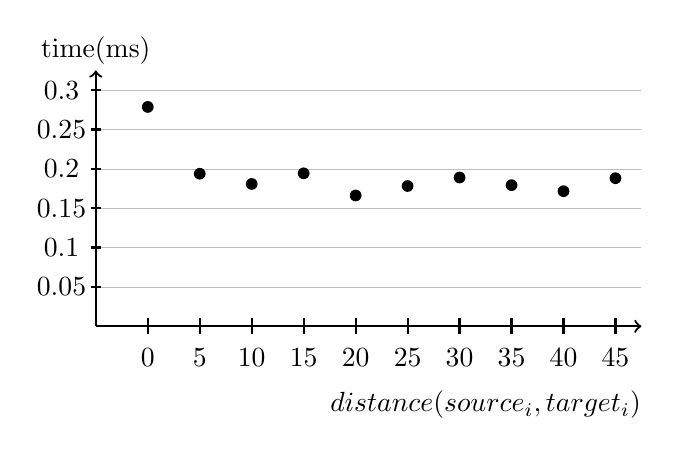
\begin{tikzpicture}[thick, yscale=10, xscale=0.66]
		%time axis
		\draw[->] (0,0) -- (0,0.325);
		\node at (0, 0.35){time(ms)};
		
		\foreach \y in {0.05, 0.1, 0.15, 0.2, 0.25, 0.3}{
			\draw[very thin, lightgray] (0, \y)--(10.5, \y);
			\draw(-0.1, \y)--(0.1, \y);
			\node at (-0.66, \y){\y};
			
		}
		
		\draw[->] (0,0) -- (10.5, 0);
		\node at (7.5, -0.1){$distance(source_i, target_{i})$};
		\foreach \x in {0, 1, 2, ..., 9}{
			\draw(\x+1, 0.01)--(\x+1, -0.01);
		}
		\node at (1, -0.04){$0$};
		\node at (2, -0.04){$5$};
		\node at (3, -0.04){$10$};
		\node at (4, -0.04){$15$};
		\node at (5, -0.04){$20$};
		\node at (6, -0.04){$25$};
		\node at (7, -0.04){$30$};
		\node at (8, -0.04){$35$};
		\node at (9, -0.04){$40$};
		\node at (10, -0.04){$45$};
		
		\node at (1, 0.2786) [circle,fill,inner sep=1.5pt]{};
		\node at (2, 0.1938) [circle,fill,inner sep=1.5pt]{};
		\node at (3, 0.1808) [circle,fill,inner sep=1.5pt]{};
		\node at (4, 0.1943) [circle,fill,inner sep=1.5pt]{};
		\node at (5, 0.1662) [circle,fill,inner sep=1.5pt]{};
		\node at (6, 0.1782) [circle,fill,inner sep=1.5pt]{};
		\node at (7, 0.189) [circle,fill,inner sep=1.5pt]{};
		\node at (8, 0.1793) [circle,fill,inner sep=1.5pt]{};
		\node at (9, 0.1716) [circle,fill,inner sep=1.5pt]{};
		\node at (10, 0.1881) [circle,fill,inner sep=1.5pt]{};
		\end{tikzpicture}
		\centering
		\caption{Average run times of the \textit{Order-\\Constraint} with a distance between subsequent\\ $source$ events of $21$ in dependency of the\\ distance $source$ events and their associated\\ $target$ event}
		\label{fig:OrderConstraintRunTime2}
	\end{minipage}
\end{figure}

\subsubsection{SporadicConstraint}
The traces, that were used for the evaluation fulfill the constraint with the parameters $jitter\in\{1,11,21,31\}$, $lower\in\{500,600,...,900\}$ and $upper=lower+x$, $x\in\{100, 200, ..., 500\}$. The average run time per timestamps of the monitor with the parameters $lower=500$ and $upper=600$ with different values for the $jitter$ parameter can be seen in Figure~\ref{fig:SporadicConstraintRuntime1}. Similar to the run times with varying $upper$ values (figure~\ref{fig:SporadicConstraintRuntime2}), the run times are nearly constant. As expected by the analysis of the implementation in the previous section, the parameters did not influence the run time.

\begin{figure}
	\centering
	\begin{minipage}{0.45\textwidth}
		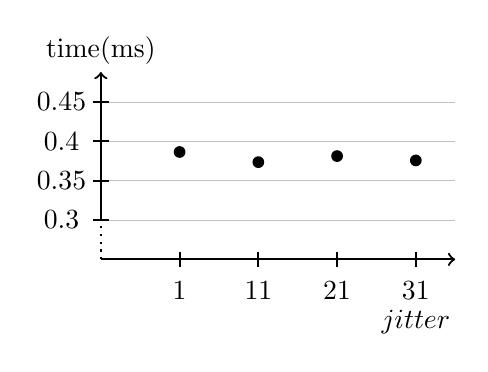
\begin{tikzpicture}[thick, yscale=10]
		%time axis
		\draw[->] (0,0.3) -- (0,0.488);
		\draw[dotted] (0, 0.25) -- (0,0.3);
		\node at (0, 0.515){time(ms)};
		
		\foreach \y in {0.3, 0.35, 0.4, 0.45}{
			\draw[very thin, lightgray] (0, \y)--(4.5, \y);
			\draw(-0.1, \y)--(0.1, \y);
			\node at (-0.5, \y){\y};
		
		}
		
		\draw[->] (0,0.25) -- (4.5, 0.25);
		\node at (4, 0.17){$jitter$};
		\foreach \x in {0, 1, 2, ..., 3}{
			\draw(\x+1, 0.26)--(\x+1, 0.24);
		}
		\node at (1, 0.21){$1$};
		\node at (2, 0.21){$11$};
		\node at (3, 0.21){$21$};
		\node at (4, 0.21){$31$};
		\node at (1, 0.3864) [circle,fill,inner sep=1.5pt]{};
		\node at (2, 0.3735) [circle,fill,inner sep=1.5pt]{};
		\node at (3, 0.3812) [circle,fill,inner sep=1.5pt]{};
		\node at (4, 0.3757) [circle,fill,inner sep=1.5pt]{};
		\end{tikzpicture}
		\centering
		\caption{Average run times of the\\ \textit{SporadicConstraint} with the\\ parameters $lower = 500, upper = 600$}
		\label{fig:SporadicConstraintRuntime1}
	\end{minipage}\hfill
	\begin{minipage}{0.45\textwidth}
		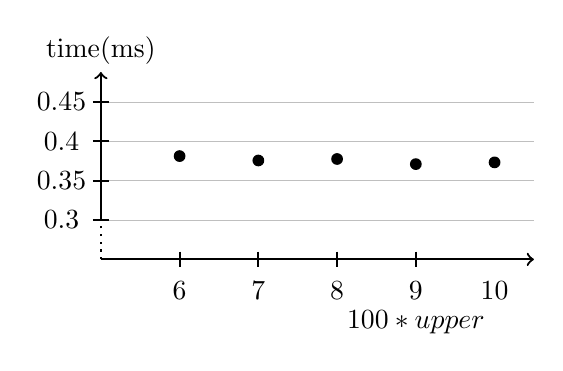
\begin{tikzpicture}[thick, yscale=10]
		%time axis
		\draw[->] (0,0.3) -- (0,0.488);
		\draw[dotted] (0, 0.25) -- (0,0.3);
		\node at (0,0.515){time(ms)};
		
		\foreach \y in {0.3, 0.35, 0.4, 0.45}{
			\draw[very thin, lightgray] (0, \y)--(5.5, \y);
			\draw(-0.1, \y)--(0.1, \y);
			\node at (-0.5, \y){\y};
		
		}
		
		\draw[->] (0,0.25) -- (5.5, 0.25);
		\node at (4, 0.17){$100*upper$};
		\foreach \x in {0, 1, 2, ..., 3}{
			\draw(\x+1, 0.26)--(\x+1, 0.24);
		}
		\node at (1, 0.21){$6$};
		\node at (2, 0.21){$7$};
		\node at (3, 0.21){$8$};
		\node at (4, 0.21){$9$};
		\node at (5, 0.21){$10$};
		\node at (1, 0.3812) [circle,fill,inner sep=1.5pt]{};
		\node at (2, 0.3756) [circle,fill,inner sep=1.5pt]{};
		\node at (3, 0.3775) [circle,fill,inner sep=1.5pt]{};
		\node at (4, 0.371) [circle,fill,inner sep=1.5pt]{};
		\node at (5, 0.3732) [circle,fill,inner sep=1.5pt]{};
		\end{tikzpicture}
		\centering
		\caption{Average run times of the\\ \textit{SporadicConstraint} with the parameters\\ $lower = 500, jitter = 21$}
		\label{fig:SporadicConstraintRuntime2}
	\end{minipage}
\end{figure}

\subsubsection{PeriodicConstraint}
The run time evaluation was done on traces, which fulfill the \textit{PeriodicConstraint} with the parameters $period\in\{10,20,30,..,100\}$ and $jitter\in\{0,1,..,9\}$. In figure~\ref{fig:PeriodicConstrainttRunTime1}, the average run times of the monitor with a constant $period$ and a variable $jitter$ can be seen, in figure~\ref{fig:PeriodicConstrainttRunTime2}, $jitter$ is fixed and $period$ is variable. Despite some fluctuations, the run time is constant and independent of the input parameters. This behavior was expected by the analysis of the source code.
\begin{figure}
	\begin{minipage}{0.45\textwidth}
		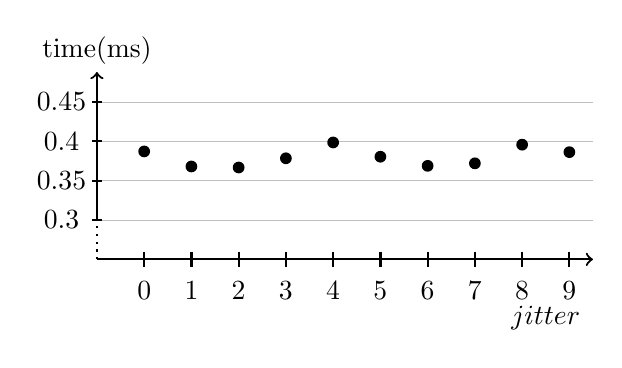
\begin{tikzpicture}[thick, yscale=10, xscale=0.6]
		%time axis
		\draw[->] (0,0.3) -- (0,0.488);
		\draw[dotted] (0, 0.25) -- (0,0.3);
		\node at (0, 0.515){time(ms)};
		
		\foreach \y in {0.3, 0.35, 0.4, 0.45}{
			\draw[very thin, lightgray] (0, \y)--(10.5, \y);
			\draw(-0.1, \y)--(0.1, \y);
			\node at (-0.75, \y){\y};
			
		}
		
		\draw[->] (0,0.25) -- (10.5, 0.25);
		\node at (9.5, 0.175){$jitter$};
		\foreach \x in {0, 1, 2, ..., 9}{
			\draw(\x+1, 0.26)--(\x+1, 0.24);
			\node at (\x+1, 0.21){$\x$};
		}
		
		\node at (1, 0.3871) [circle,fill,inner sep=1.5pt]{};
		\node at (2, 0.368) [circle,fill,inner sep=1.5pt]{};
		\node at (3, 0.3667) [circle,fill,inner sep=1.5pt]{};
		\node at (4, 0.3784) [circle,fill,inner sep=1.5pt]{};
		\node at (5, 0.3985) [circle,fill,inner sep=1.5pt]{};
		\node at (6, 0.3804) [circle,fill,inner sep=1.5pt]{};
		\node at (7, 0.3688) [circle,fill,inner sep=1.5pt]{};
		\node at (8, 0.372) [circle,fill,inner sep=1.5pt]{};
		\node at (9, 0.3957) [circle,fill,inner sep=1.5pt]{};
		\node at (10, 0.3862) [circle,fill,inner sep=1.5pt]{};
		\end{tikzpicture}
		\centering
		\caption{Average run times of the \\\textit{PeriodicConstraint} with a $period$ of 70 and\\ variable $jitter$}
		\label{fig:PeriodicConstrainttRunTime1}
	\end{minipage}\hfill
	\begin{minipage}{0.45\textwidth}
		\centering
		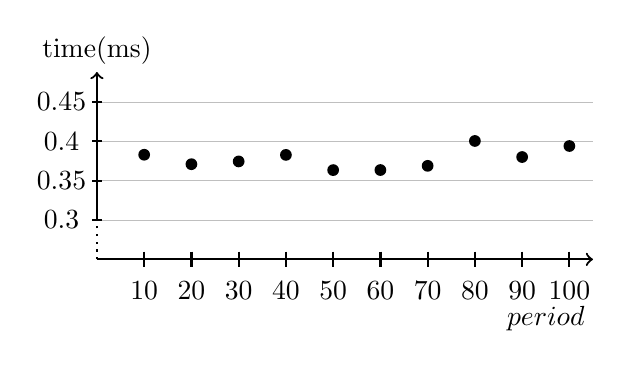
\begin{tikzpicture}[thick, yscale=10, xscale=0.6]
		%time axis
		\draw[->] (0,0.3) -- (0,0.488);
		\draw[dotted] (0, 0.25) -- (0,0.3);
		\node at (0, 0.515){time(ms)};
		
		\foreach \y in {0.3, 0.35, 0.4, 0.45}{
			\draw[very thin, lightgray] (0, \y)--(10.5, \y);
			\draw(-0.1, \y)--(0.1, \y);
			\node at (-0.75, \y){\y};
			
		}
		
		\draw[->] (0,0.25) -- (10.5, 0.25);
		\node at (9.5, 0.175){$period$};
		\foreach \x in {0, 1, 2, ..., 9}{
			\draw(\x+1, 0.26)--(\x+1, 0.24);
			%\node at (\x+1, 0.21){$\x0$};
		}
		\foreach \x in {1, 2, ..., 10}{
			\node at (\x, 0.21){$\x0$};
		}
		\node at (1, 0.3829) [circle,fill,inner sep=1.5pt]{};
		\node at (2, 0.3709) [circle,fill,inner sep=1.5pt]{};
		\node at (3, 0.3744) [circle,fill,inner sep=1.5pt]{};
		\node at (4, 0.3827) [circle,fill,inner sep=1.5pt]{};
		\node at (5, 0.3634) [circle,fill,inner sep=1.5pt]{};
		\node at (6, 0.3635) [circle,fill,inner sep=1.5pt]{};
		\node at (7, 0.3688) [circle,fill,inner sep=1.5pt]{};
		\node at (8, 0.4004) [circle,fill,inner sep=1.5pt]{};
		\node at (9, 0.38) [circle,fill,inner sep=1.5pt]{};
		\node at (10, 0.394) [circle,fill,inner sep=1.5pt]{};
		\end{tikzpicture}
		\centering
		\caption{Average run times of the \textit{Periodic-\\Constraint} with a $jitter$ of 6 and variable $period$}
		\label{fig:PeriodicConstrainttRunTime2}
	\end{minipage}
\end{figure}



\subsubsection{PatternConstraint}
	The monitor of the \emph{PatternConstraint} was first evaluated on traces with lengths of the $|$\textit{offset}$|$ parameter of 1, 2 and 3 and varying values for the parameters $period$ and $jitter$. Also, the values inside of $|$\textit{offset}$|$ were changing. Figure~\ref{fig:PatternConstraintTimeMeasure1} and \ref{fig:PatternConstraintTimeMeasure2} show some of these results, which were nearly constant at around 0.65ms per input timestamp. After these run time measurements, the run time was measured on traces with the parameters $jitter=0$ and $period=200$. The \textit{offset} parameter had an increasing length from 1 to 100 and was filled with \textit{offset}$=[0, 1, 2, 3, ...]$. The results of this measurement can be seen in figure~\ref{fig:PatternConstraintTimeMeasure3}. It can be seen that the average run times were nearly constant, besides some measurement deviations. This behavior was expected by the analysis in the previous section.
	
	\begin{figure}
		\centering
		\begin{minipage}{0.45\textwidth}
			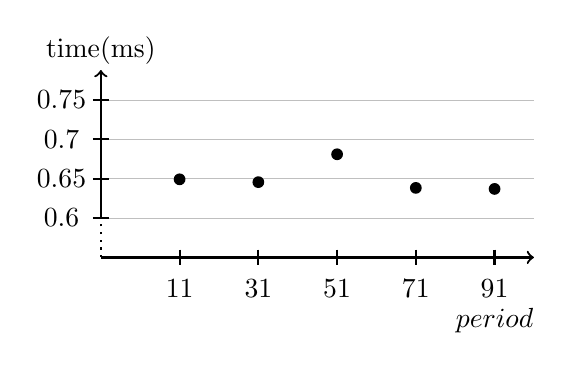
\begin{tikzpicture}[thick, yscale=10]
				%time axis
				\draw[->] (0,0.6) -- (0,0.788);
				\draw[dotted] (0, 0.55) -- (0,0.6);
				\node at (0, 0.8125){time(ms)};
				
				\foreach \y in {0.6, 0.65, 0.7, 0.75}{
					\draw[very thin, lightgray] (0, \y)--(5.5, \y);
					\draw(-0.1, \y)--(0.1, \y);
					\node at (-0.5, \y){\y};
				
				}
				
				\draw[->] (0,0.55) -- (5.5, 0.55);
				\node at (5, 0.47){$period$};
				\foreach \x in {0, 1, 2, ..., 3, 4}{
					\draw(\x+1, 0.56)--(\x+1, 0.54);
				}
				\node at (1, 0.51){$11$};
				\node at (2, 0.51){$31$};
				\node at (3, 0.51){$51$};
				\node at (4, 0.51){$71$};
				\node at (5, 0.51){$91$};
				\node at (1, 0.6492) [circle,fill,inner sep=1.5pt]{};
				\node at (2, 0.6456) [circle,fill,inner sep=1.5pt]{};
				\node at (3, 0.681) [circle,fill,inner sep=1.5pt]{};
				\node at (4, 0.6383) [circle,fill,inner sep=1.5pt]{};
				\node at (5, 0.637) [circle,fill,inner sep=1.5pt]{};
			\end{tikzpicture}
			\centering
			\caption{Average run times of the\\ \textit{PatternConstraint} with the parameters\\ \textit{offset}$ = [0,1]$ and $jitter = 0$}
			\label{fig:PatternConstraintTimeMeasure1}
		\end{minipage}\hfill
		\begin{minipage}{0.45\textwidth}
			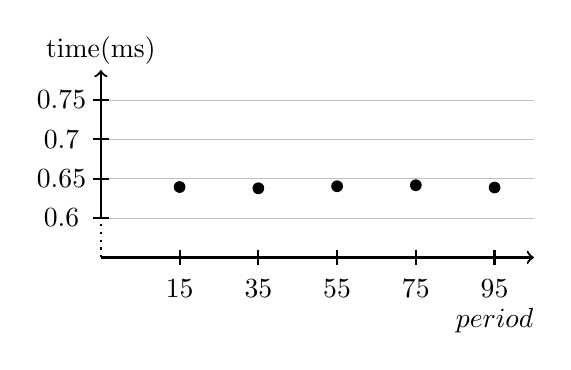
\begin{tikzpicture}[thick, yscale=10]
				%time axis
				\draw[->] (0,0.6) -- (0,0.788);
				\draw[dotted] (0, 0.55) -- (0,0.6);
				\node at (0, 0.8125){time(ms)};
				
				\foreach \y in {0.6, 0.65, 0.7, 0.75}{
					\draw[very thin, lightgray] (0, \y)--(5.5, \y);
					\draw(-0.1, \y)--(0.1, \y);
					\node at (-0.5, \y){\y};
					
				}
				
				\draw[->] (0,0.55) -- (5.5, 0.55);
				\node at (5, 0.47){$period$};
				\foreach \x in {0, 1, 2, ..., 3, 4}{
					\draw(\x+1, 0.56)--(\x+1, 0.54);
				}
				\node at (1, 0.51){$15$};
				\node at (2, 0.51){$35$};
				\node at (3, 0.51){$55$};
				\node at (4, 0.51){$75$};
				\node at (5, 0.51){$95$};
				\node at (1, 0.6394) [circle,fill,inner sep=1.5pt]{};
				\node at (2, 0.6378) [circle,fill,inner sep=1.5pt]{};
				\node at (3, 0.6404) [circle,fill,inner sep=1.5pt]{};
				\node at (4, 0.6417) [circle,fill,inner sep=1.5pt]{};
				\node at (5, 0.6388) [circle,fill,inner sep=1.5pt]{};
			\end{tikzpicture}
			\centering
			\caption{Average run times of the\\ \textit{PatternConstraint} with the parameters\\ \textit{offset} = $[1,3,5]$ and $jitter = 1$}
			\label{fig:PatternConstraintTimeMeasure2}
		\end{minipage}
	\end{figure}

\begin{figure}
	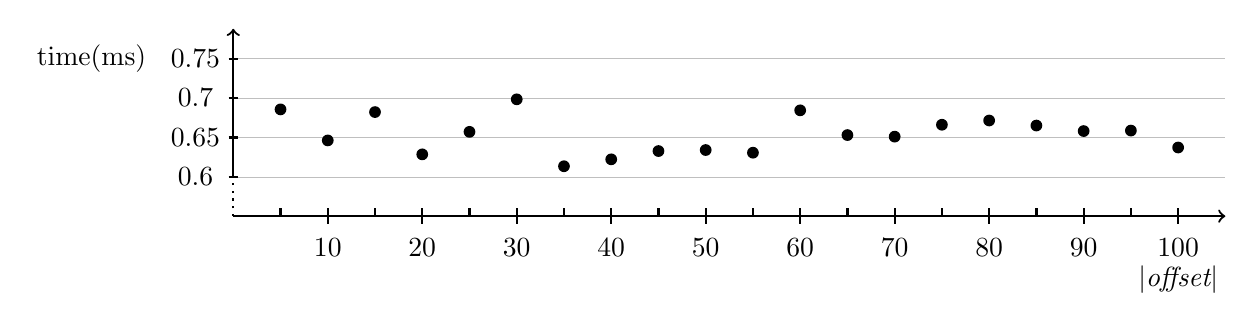
\begin{tikzpicture}[thick, yscale=10, xscale=0.12]
	%time axis
	\draw[->] (0,0.6) -- (0,0.788);
	\draw[dotted] (0, 0.55) -- (0,0.6);
	\node at (-15, 0.75){time(ms)};
	
	\foreach \y in { 0.6, 0.65, 0.7, 0.75}{
		\draw[very thin, lightgray] (0, \y)--(105, \y);
		\draw(-0.5, \y)--(0.5, \y);
		\node at (-4, \y){\y};
	}
	
	\draw[->] (0,0.55) -- (105, 0.55);
	\node at (100, 0.47){$|\text{\textit{offset}}|$};
	\foreach \x in {10, 20, ..., 90}{
		\draw(\x, 0.56)--(\x, 0.54);
		\node at (\x, 0.51){$\x$};
		\draw(\x+5, 0.56)--(\x+5, 0.55);
	}
	\draw(100, 0.56)--(100, 0.54);
	\draw(5, 0.56)--(5, 0.55);
	\node at (100, 0.51){100};
	
	\node at (5, 0.6856) [circle,fill,inner sep=1.5pt]{};
	\node at (10, 0.6462) [circle,fill,inner sep=1.5pt]{};
	\node at (15, 0.6822) [circle,fill,inner sep=1.5pt]{};
	\node at (20, 0.6285) [circle,fill,inner sep=1.5pt]{};
	\node at (25, 0.6571) [circle,fill,inner sep=1.5pt]{};
	\node at (30, 0.6984) [circle,fill,inner sep=1.5pt]{};
	\node at (35, 0.6134) [circle,fill,inner sep=1.5pt]{};
	\node at (40, 0.6222) [circle,fill,inner sep=1.5pt]{};
	\node at (45, 0.6327) [circle,fill,inner sep=1.5pt]{};
	\node at (50, 0.634) [circle,fill,inner sep=1.5pt]{};
	\node at (55, 0.6306) [circle,fill,inner sep=1.5pt]{};
	\node at (60, 0.6844) [circle,fill,inner sep=1.5pt]{};
	\node at (65, 0.653) [circle,fill,inner sep=1.5pt]{};
	\node at (70, 0.651) [circle,fill,inner sep=1.5pt]{};
	\node at (75, 0.6661) [circle,fill,inner sep=1.5pt]{};
	\node at (80, 0.6715) [circle,fill,inner sep=1.5pt]{};
	\node at (85, 0.6651) [circle,fill,inner sep=1.5pt]{};
	\node at (90, 0.6581) [circle,fill,inner sep=1.5pt]{};
	\node at (95, 0.6587) [circle,fill,inner sep=1.5pt]{};
	\node at (100, 0.6372) [circle,fill,inner sep=1.5pt]{};

	\end{tikzpicture}
	\centering
	\caption{Average run times of the \textit{PatternConstraint} with the parameters \textit{period} $= 200$ and $jitter = 0$}
	\label{fig:PatternConstraintTimeMeasure3}
\end{figure}


\subsubsection{ArbitraryConstraint}
	Similar to the previous constraint, multiple runs were done for the run time measurement. First, with small lengths of the $minimum$ and $maximum$ parameter and changing values for the values inside of these parameters, and then with a length of the $minimum$ and $maximum$ parameter of 1 to 60. Figure~\ref{fig:ArbitraryConstraintTimeMeasure1} and \ref{fig:ArbitraryConstraintTimeMeasure2} are showing some of the results with short $minimum$ and $maximum$ parameters. It can be seen that the results with the same length of these parameters are nearly constant, but the traces with a $minimum$ length of 3 took slightly more time. Figure~\ref{fig:ArbitraryConstraintTimeMeasure3} shows the average run times in dependency of the length of the $minimum$ parameter. The graphic shows a linear growth of the run time, which matches the expectation in the analysis.
	\begin{figure}
	\centering
	\begin{minipage}{0.45\textwidth}
		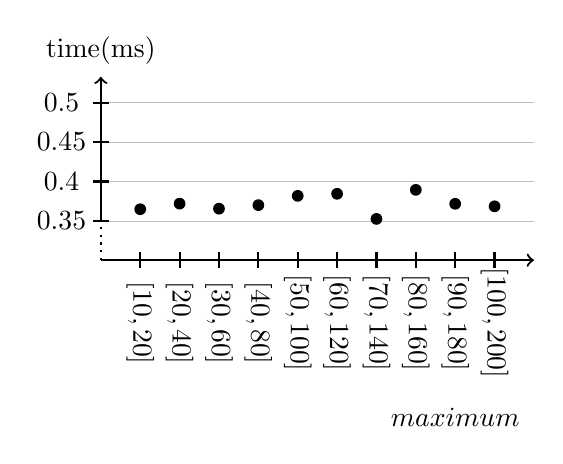
\begin{tikzpicture}[thick, yscale=10]
		%time axis
		\draw[->] (0.5,0.35) -- (0.5,0.533);
		\draw[dotted] (0.5, 0.3) -- (0.5,0.35);
		\node at (0.5, 0.566){time(ms)};
		
		\foreach \y in {0.35, 0.4, 0.45, 0.5}{
			\draw[very thin, lightgray] (0.5, \y)--(6, \y);
			\draw(0.4, \y)--(0.6, \y);
			\node at (0, \y){\y};
			
		}
		
		\draw[->] (0.5,0.3) -- (6, 0.3);
		\node at (5, 0.1){$maximum$};
		\foreach \x in {0, 0.5, 1, ..., 4.5}{
			\draw(\x+1, 0.31)--(\x+1, 0.29);
		}
		\node[rotate=270] at (1, 0.22){$[10,20]$};
		\node[rotate=270] at (1.5, 0.22){$[20,40]$};
		\node[rotate=270] at (2, 0.22){$[30,60]$};
		\node[rotate=270] at (2.5, 0.22){$[40,80]$};
		\node[rotate=270] at (3, 0.22){$[50,100]$};
		\node[rotate=270] at (3.5, 0.22){$[60,120]$};
		\node[rotate=270] at (4, 0.22){$[70,140]$};
		\node[rotate=270] at (4.5, 0.22){$[80,160]$};
		\node[rotate=270] at (5, 0.22){$[90,180]$};
		\node[rotate=270] at (5.5, 0.22){$[100,200]$};
		\node at (1, 0.3647) [circle,fill,inner sep=1.5pt]{};
		\node at (1.5, 0.3718) [circle,fill,inner sep=1.5pt]{};
		\node at (2, 0.3654) [circle,fill,inner sep=1.5pt]{};
		\node at (2.5, 0.3699) [circle,fill,inner sep=1.5pt]{};
		\node at (3, 0.3817) [circle,fill,inner sep=1.5pt]{};
		\node at (3.5, 0.3843) [circle,fill,inner sep=1.5pt]{};
		\node at (4, 0.3524) [circle,fill,inner sep=1.5pt]{};
		\node at (4.5, 0.3893) [circle,fill,inner sep=1.5pt]{};
		\node at (5, 0.3716) [circle,fill,inner sep=1.5pt]{};
		\node at (5.5, 0.3684) [circle,fill,inner sep=1.5pt]{};
		\end{tikzpicture}
		\centering
		\caption{Average run times of the\\ \textit{ArbitraryConstraint} with the\\ parameter $minimum = [10,20]$}
		\label{fig:ArbitraryConstraintTimeMeasure1}
	\end{minipage}\hfill
	\begin{minipage}{0.45\textwidth}
		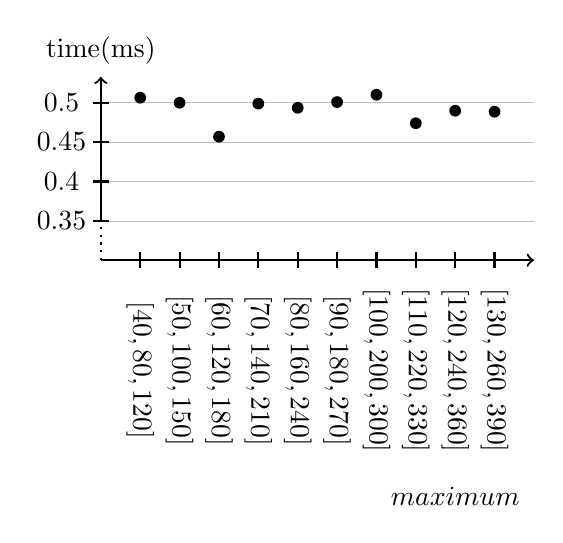
\begin{tikzpicture}[thick, yscale=10]
			%time axis
			\draw[->] (0.5,0.35) -- (0.5,0.533);
			\draw[dotted] (0.5, 0.3) -- (0.5,0.35);
			\node at (0.5, 0.566){time(ms)};
			
			\foreach \y in {0.35, 0.4, 0.45, 0.5}{
				\draw[very thin, lightgray] (0.5, \y)--(6, \y);
				\draw(0.4, \y)--(0.6, \y);
				\node at (0, \y){\y};
				
			}
			
			\draw[->] (0.5,0.3) -- (6, 0.3);
			\node at (5, 0.0){$maximum$};
			\foreach \x in {0, 0.5, 1, ..., 4.5}{
				\draw(\x+1, 0.31)--(\x+1, 0.29);
			}
			\node[rotate=270] at (1, 0.16)	{$[40 ,80 ,120]$};
			\node[rotate=270] at (1.5, 0.16){$[50 ,100 ,150]$};
			\node[rotate=270] at (2, 0.16)	{$[60 ,120,180]$};
			\node[rotate=270] at (2.5, 0.16){$[70 ,140,210]$};
			\node[rotate=270] at (3, 0.16)	{$[80 ,160,240]$};
			\node[rotate=270] at (3.5, 0.16){$[90 ,180,270]$};
			\node[rotate=270] at (4, 0.16)	{$[100 ,200,300]$};
			\node[rotate=270] at (4.5, 0.16){$[110,220,330]$};
			\node[rotate=270] at (5, 0.16)	{$[120,240,360]$};
			\node[rotate=270] at (5.5, 0.16){$[130,260,390]$};
			\node at (1, 0.5063) [circle,fill,inner sep=1.5pt]{};
			\node at (1.5, 0.4999) [circle,fill,inner sep=1.5pt]{};
			\node at (2, 0.4568) [circle,fill,inner sep=1.5pt]{};
			\node at (2.5, 0.4988) [circle,fill,inner sep=1.5pt]{};
			\node at (3, 0.4935) [circle,fill,inner sep=1.5pt]{};
			\node at (3.5, 0.5008) [circle,fill,inner sep=1.5pt]{};
			\node at (4, 0.5101) [circle,fill,inner sep=1.5pt]{};
			\node at (4.5, 0.4739) [circle,fill,inner sep=1.5pt]{};
			\node at (5, 0.4898) [circle,fill,inner sep=1.5pt]{};
			\node at (5.5, 0.4886) [circle,fill,inner sep=1.5pt]{};
		\end{tikzpicture}
		\centering
		\caption{Average run times of the\\ \textit{ArbitraryConstraint} with the\\ parameter $minimum = [40,80, 120]$}
		\label{fig:ArbitraryConstraintTimeMeasure2}
	\end{minipage}
\end{figure}

\begin{figure}
	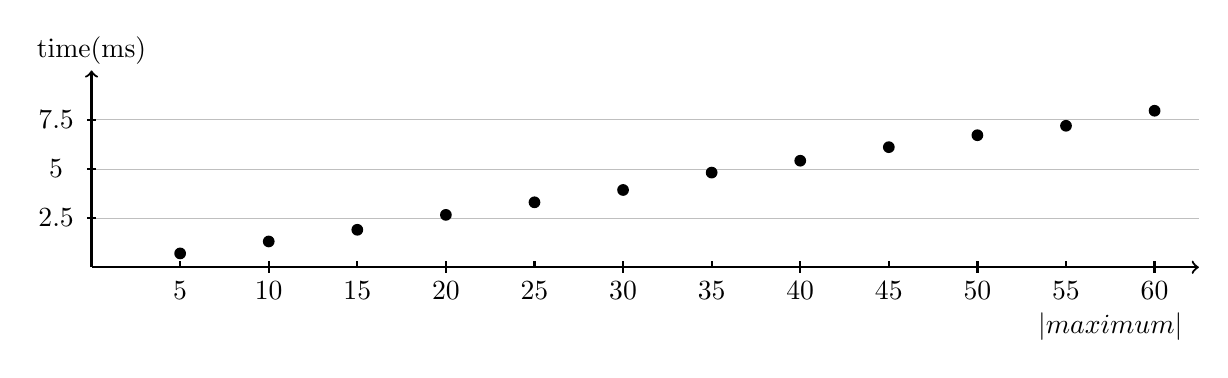
\begin{tikzpicture}[thick, yscale=0.25, xscale=0.225]
	%time axis
	\draw[->] (0,0.0) -- (0,10);
	\node at (0, 11){time(ms)};
	
	\foreach \y in {2.5, 5, 7.5}{
		\draw[very thin, lightgray] (0, \y)--(62.5, \y);
		\draw(-0.25, \y)--(0.25, \y);
		\node at (-2, \y){\y};
	}
	
	\draw[->] (0,0.0) -- (62.5, 0.0);
	\node at (57.5, -3){$|maximum|$};
	\foreach \x in {10, 20, ..., 50}{
		\draw(\x, .3)--(\x, -.3);
		\draw(\x+5, .3)--(\x+5, 0.0);
	}
	\draw(0+5, .3)--(0+5, 0.0);
	\draw(60, .3)--(60, -.3);
	
	\node at (5, -1.2){5};
	\node at (10, -1.2){10};
	\node at (15, -1.2){15};
	\node at (20, -1.2){20};
	\node at (25, -1.2){25};
	\node at (30, -1.2){30};
	\node at (35, -1.2){35};
	\node at (40, -1.2){40};
	\node at (45, -1.2){45};
	\node at (50, -1.2){50};
	\node at (55, -1.2){55};
	\node at (60, -1.2){60};
	
	\node at (5, 0.7037) [circle,fill,inner sep=1.5pt]{};
	\node at (10, 1.3108) [circle,fill,inner sep=1.5pt]{};
	\node at (15, 1.9042) [circle,fill,inner sep=1.5pt]{};
	\node at (20, 2.6612) [circle,fill,inner sep=1.5pt]{};
	\node at (25, 3.3003) [circle,fill,inner sep=1.5pt]{};
	\node at (30, 3.9266) [circle,fill,inner sep=1.5pt]{};
	\node at (35, 4.8095) [circle,fill,inner sep=1.5pt]{};
	\node at (40, 5.4126) [circle,fill,inner sep=1.5pt]{};
	\node at (45, 6.1017) [circle,fill,inner sep=1.5pt]{};
	\node at (50, 6.7075) [circle,fill,inner sep=1.5pt]{};
	\node at (55, 7.1881) [circle,fill,inner sep=1.5pt]{};
	\node at (60, 7.9516) [circle,fill,inner sep=1.5pt]{};

	
	\end{tikzpicture}
	\centering
	\caption{Average run times of the \textit{ArbitraryConstraint} with $|maximum|=1..60$}
	\label{fig:ArbitraryConstraintTimeMeasure3}
\end{figure}
	

\subsubsection{BurstConstraint}
	Figure~\ref{fig:BurstConstraintRunTime} shows the average run time per input timestamp with increasing the number of occurrences per burst. The runtime was nearly constant, which was expected because the \textit{BurstConstraint} is defined as an application of the \textit{RepeatConstraint}, which also has a constant run time.
\begin{figure}
	\centering
	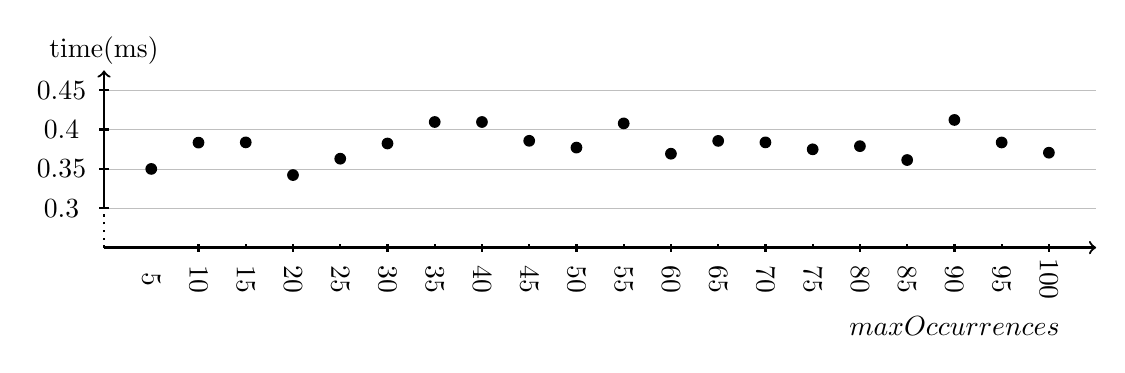
\begin{tikzpicture}[thick, yscale=10, xscale=1.2]
	%time axis
	\draw[->] (0,0.3) -- (0,0.475);
	\draw[dotted] (0, 0.25) -- (0,0.3);
	\node at (0, 0.5){time(ms)};
	
	\foreach \y in {0.3, 0.35, 0.4, 0.45}{
		\draw[very thin, lightgray] (0, \y)--(10.5, \y);
		\draw(-0.05, \y)--(0.05, \y);
		\node at (-0.45, \y){\y};
		
	}
	
	\draw[->] (0,0.25) -- (10.5, 0.25);
	\node at (9, 0.15){$maxOccurrences$};
	\foreach \x in {1, 2, ..., 9}{
		\draw(\x, 0.245)--(\x, 0.255);
		\draw(\x+0.5, 0.25)--(\x+0.5, 0.255);
		%\node at (\x+1, 0.21){$\x0$};
	}
	\draw(10, 0.245)--(10, 0.255);

	\node[rotate=270] at (0.5, 0.21){$5$};
	\node[rotate=270] at (1, 0.21){$10$};
	\node[rotate=270] at (1.5, 0.21){$15$};
	\node[rotate=270] at (2, 0.21){$20$};
	\node[rotate=270] at (2.5, 0.21){$25$};
	\node[rotate=270] at (3, 0.21){$30$};
	\node[rotate=270] at (3.5, 0.21){$35$};
	\node[rotate=270] at (4, 0.21){$40$};
	\node[rotate=270] at (4.5, 0.21){$45$};
	\node[rotate=270] at (5, 0.21){$50$};
	\node[rotate=270] at (5.5, 0.21){$55$};
	\node[rotate=270] at (6, 0.21){$60$};
	\node[rotate=270] at (6.5, 0.21){$65$};
	\node[rotate=270] at (7, 0.21){$70$};
	\node[rotate=270] at (7.5, 0.21){$75$};
	\node[rotate=270] at (8, 0.21){$80$};
	\node[rotate=270] at (8.5, 0.21){$85$};
	\node[rotate=270] at (9, 0.21){$90$};
	\node[rotate=270] at (9.5, 0.21){$95$};
	\node[rotate=270] at (10, 0.21){$100$};


	\node at (0.5, 0.3499) [circle,fill,inner sep=1.5pt]{};
	\node at (1, 0.3833) [circle,fill,inner sep=1.5pt]{};
	\node at (1.5, 0.3836) [circle,fill,inner sep=1.5pt]{};
	\node at (2, 0.3421) [circle,fill,inner sep=1.5pt]{};
	\node at (2.5, 0.3629) [circle,fill,inner sep=1.5pt]{};
	\node at (3, 0.3822) [circle,fill,inner sep=1.5pt]{};
	\node at (3.5, 0.4095) [circle,fill,inner sep=1.5pt]{};
	\node at (4, 0.4095) [circle,fill,inner sep=1.5pt]{};
	\node at (4.5, 0.3856) [circle,fill,inner sep=1.5pt]{};
	\node at (5, 0.377) [circle,fill,inner sep=1.5pt]{};
	\node at (5.5, 0.4077) [circle,fill,inner sep=1.5pt]{};
	\node at (6, 0.3692) [circle,fill,inner sep=1.5pt]{};
	\node at (6.5, 0.3855) [circle,fill,inner sep=1.5pt]{};
	\node at (7, 0.3836) [circle,fill,inner sep=1.5pt]{};
	\node at (7.5, 0.3748) [circle,fill,inner sep=1.5pt]{};
	\node at (8, 0.3788) [circle,fill,inner sep=1.5pt]{};
	\node at (8.5, 0.3612) [circle,fill,inner sep=1.5pt]{};
	\node at (9, 0.4121) [circle,fill,inner sep=1.5pt]{};
	\node at (9.5, 0.3835) [circle,fill,inner sep=1.5pt]{};
	\node at (10, 0.3705) [circle,fill,inner sep=1.5pt]{};
	\end{tikzpicture}
	\centering
	\caption{Average run times of the \textit{BurstConstraint} with increasing $occurrences$ per burst and a length of 2000}
	\label{fig:BurstConstraintRunTime}
\end{figure}

\subsubsection{ReactionConstraint}
The runtime evaluation of the \textit{ReactionConstraint} was done on traces with the parameters $minimum\in\{100,200,...,1000\}$ and $maximum = minimum$, while the distances between subsequent $stimulus$ event were in $\{1, 2, 4, 8, ..., 1024\}$, so that $minimum$, $\lceil\frac{minimum}{2}\rceil$,  $\lceil\frac{minimum}{4}\rceil$, ...,  $\lceil\frac{minimum}{1024}\rceil$ events must be stored and considered at every event in the monitor.\\
Figure~\ref{fig:ReactionConstraintRunTime1} and \ref{fig:ReactionConstraintRunTime2} are showing the average run times of the monitor with increasing $minimum$ and $maximum$ parameters but a fixed distance between subsequent $stimulus$ events. The first figure shows the run times with $stimulus$ distances of 1, which is the worst-case because $maximum$ events must be stored and considered for the correct decision of the monitor. As expected by the analysis, the run time is increasing linearly with larger $maximum$ values. This behavior can also be seen in the second figure, where the distance between the events is 64, but the run times are much shorter here. This is because between 2 ($\lceil \frac{100}{64}\rceil$) and 16 ($\lceil \frac{1000}{64}\rceil$) were considered in each timestamp with events, not between 100 and 1000 in the previous case.
\begin{figure}
	\begin{minipage}{0.45\textwidth}
		\centering
		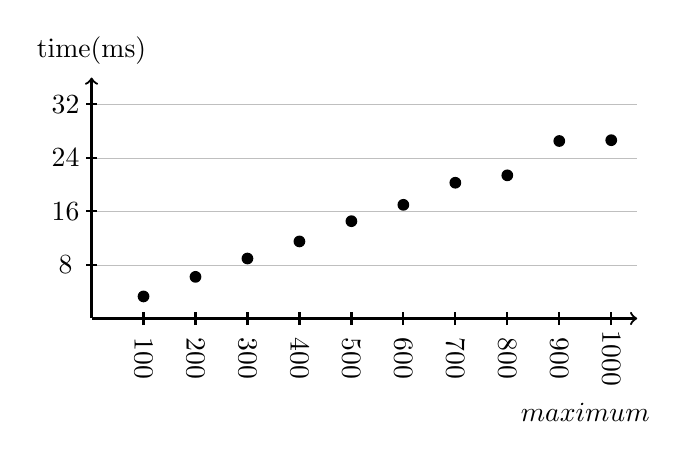
\begin{tikzpicture}[thick, yscale=0.085, xscale=0.66]
			%time axis
			\draw[->] (0,0) -- (0,36);
			\node at (0, 40){time(ms)};
			
			\foreach \y in {8,16, 24, 32}{
				\draw[very thin, lightgray] (0, \y)--(10.5, \y);
				\draw(-0.1, \y)--(0.1, \y);
				\node at (-0.5, \y){\y};
				
			}
			
			\draw[->] (0,0) -- (10.5, 0.0);
			\node at (9.5, -14){$maximum$};
			\foreach \x in {1, 2, ..., 9, 10}{
				\draw(\x, -1)--(\x, 1);
				\node[rotate=270] at (\x, -6){$\x00$};
			}
			\node at (1, 3.2912) [circle,fill,inner sep=1.5pt]{};
			\node at (2, 6.2172) [circle,fill,inner sep=1.5pt]{};
			\node at (3, 8.9579) [circle,fill,inner sep=1.5pt]{};
			\node at (4, 11.5083) [circle,fill,inner sep=1.5pt]{};
			\node at (5, 14.5341) [circle,fill,inner sep=1.5pt]{};
			\node at (6, 16.9773) [circle,fill,inner sep=1.5pt]{};
			\node at (7, 20.2771) [circle,fill,inner sep=1.5pt]{};
			\node at (8, 21.3825) [circle,fill,inner sep=1.5pt]{};
			\node at (9, 26.5124) [circle,fill,inner sep=1.5pt]{};
			\node at (10, 26.634) [circle,fill,inner sep=1.5pt]{};
		\end{tikzpicture}
		\centering
		\caption{Average run times of the \textit{Reac-\\tionConstraint} with a distance between\\ subsequent $stimulus$ events of 1 (worst case)\\ and variable $maximum$}
		\label{fig:ReactionConstraintRunTime1}
	\end{minipage}\hfill
	\begin{minipage}{0.45\textwidth}
		\centering
		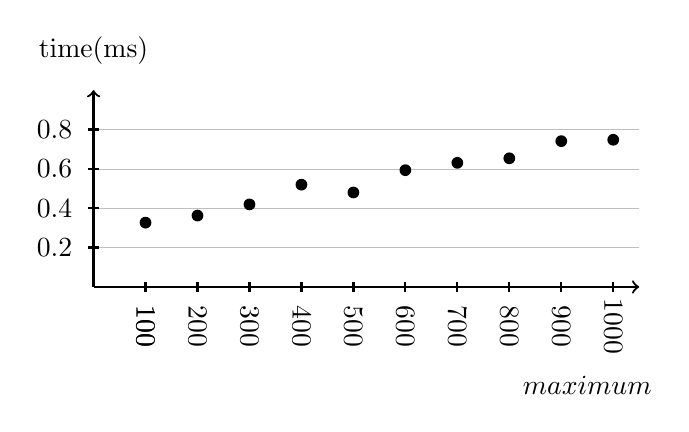
\begin{tikzpicture}[thick, yscale=2.5, xscale=0.66]
			\draw[->] (0,0) -- (0,1);
			\node at (0, 1.2){time(ms)};
			
			\foreach \y in {0.2, 0.4, 0.6, 0.8}{
				\draw[very thin, lightgray] (0, \y)--(10.5, \y);
				\draw(-0.1, \y)--(0.1, \y);
				\node at (-0.75, \y){\y};
				
			}
			
			\draw[->] (0,0.0) -- (10.5, 0.0);
			\node at (9.5, -0.5){$maximum$};
			\foreach \x in {1, 1, 2, ..., 10}{
				\draw(\x, 0.025)--(\x, -0.025);
				\node[rotate=270] at (\x, -0.2){$\x00$};
			}
			\node at (1, 0.3267) [ circle,fill,inner sep=1.5pt]{};
			\node at (2, 0.3628) [ circle,fill,inner sep=1.5pt]{};
			\node at (3, 0.4193) [ circle,fill,inner sep=1.5pt]{};
			\node at (4, 0.5197) [ circle,fill,inner sep=1.5pt]{};
			\node at (5, 0.4799) [ circle,fill,inner sep=1.5pt]{};
			\node at (6, 0.5933) [ circle,fill,inner sep=1.5pt]{};
			\node at (7, 0.6306) [ circle,fill,inner sep=1.5pt]{};
			\node at (8, 0.6536) [ circle,fill,inner sep=1.5pt]{};
			\node at (9, 0.7407) [ circle,fill,inner sep=1.5pt]{};
			\node at (10, 0.7477) [ circle,fill,inner sep=1.5pt]{};
		\end{tikzpicture}
		\centering
		\caption{Average run times of the\\\textit{ReactionConstraint} with a distance between\\ subsequent $stimulus$ events of 64 and\\ variable $maximum$}
		\label{fig:ReactionConstraintRunTime2}
	\end{minipage}
\end{figure}



\subsubsection{AgeConstraint}
The run time of the \textit{AgeConstraint} monitor was measured on traces with the same parameters as the previous constraint. Figure~\ref{fig:AgeConstraintRunTime1} shows the run times with event distances of 1, which is the worst case in terms of monitoring, in dependency of the $maximum$ parameter. With increasing $maximum$ values, the average run time grew linear, like expected in the analysis. The average run times with the same $maximum$ values and a distance between subsequent $stimulus$ events of 64 are shown in figure~\ref{fig:AgeConstraintRunTime2}. The run time is growing nearly linear again, but smaller, because only between 2 and 6 events had to be considered in each timestamp, not between 1 and 1000 like before.
\begin{figure}
	\begin{minipage}{0.45\textwidth}
		\centering
		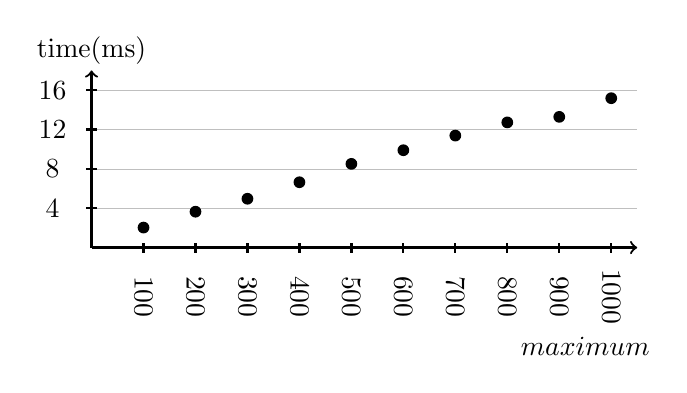
\begin{tikzpicture}[thick, yscale=0.125, xscale=0.66]
			%time axis
			\draw[->] (0,0) -- (0,18);
			\node at (0, 20){time(ms)};
			
			\foreach \y in {4, 8, ..., 16}{
				\draw[very thin, lightgray] (0, \y)--(10.5, \y);
				\draw(-0.1, \y)--(0.1, \y);
				\node at (-0.75, \y){\y};
				
			}
			
			\draw[->] (0,0) -- (10.5, 0.0);
			\node at (9.5, -10){$maximum$};
			\foreach \x in {1, 2, ..., 9, 10}{
				\draw(\x, -0.5)--(\x, 0.5);
				\node[rotate=270] at (\x, -5){$\x00$};
			}
			\node at (1, 2.0331) [circle,fill,inner sep=1.5pt]{};
			\node at (2, 3.6468) [circle,fill,inner sep=1.5pt]{};
			\node at (3, 4.9616) [circle,fill,inner sep=1.5pt]{};
			\node at (4, 6.6394) [circle,fill,inner sep=1.5pt]{};
			\node at (5, 8.5057) [circle,fill,inner sep=1.5pt]{};
			\node at (6, 9.8917) [circle,fill,inner sep=1.5pt]{};
			\node at (7, 11.3779) [circle,fill,inner sep=1.5pt]{};
			\node at (8, 12.7195) [circle,fill,inner sep=1.5pt]{};
			\node at (9, 13.2806) [circle,fill,inner sep=1.5pt]{};
			\node at (10, 15.1759) [circle,fill,inner sep=1.5pt]{};
		\end{tikzpicture}
		\centering
		\caption{Average run times of the\\ \textit{AgeConstraint} with a distance between\\ subsequent $stimulus$ events of 1 (worst case)\\  and variable $maximum$}
		\label{fig:AgeConstraintRunTime1}
	\end{minipage} \hfill
	\begin{minipage}{0.45\textwidth}
		\centering
		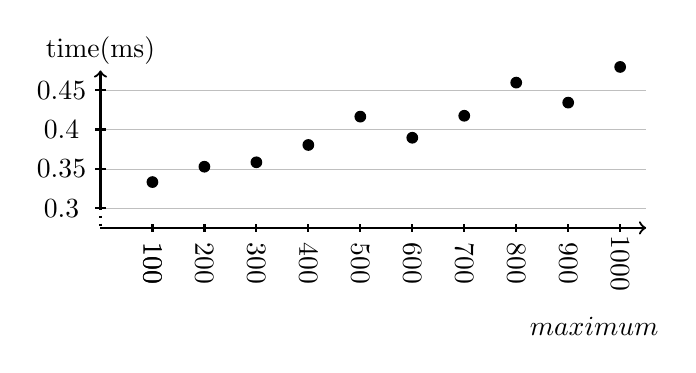
\begin{tikzpicture}[thick, yscale=10, xscale=0.66]
			\draw[->] (0,.3) -- (0,.475);
			\draw[dotted] (0, .3) -- (0,0.275);
			\node at (0, 0.5){time(ms)};
			
			\foreach \y in {0.3, 0.35, 0.4, 0.45}{
				\draw[very thin, lightgray] (0, \y)--(10.5, \y);
				\draw(-0.1, \y)--(0.1, \y);
				\node at (-0.75, \y){\y};
				
			}
			
			\draw[->] (0,0.275) -- (10.5, 0.275);
			\node at (9.5, 0.15){$maximum$};
			\foreach \x in {1, 1, 2, ..., 10}{
				\draw(\x, 0.27)--(\x, 0.28);
				\node[rotate=270] at (\x, 0.23){$\x00$};
			}
			\node at (1, 0.3332) [ circle,fill,inner sep=1.5pt]{};
			\node at (2, 0.3527) [ circle,fill,inner sep=1.5pt]{};
			\node at (3, 0.3583) [ circle,fill,inner sep=1.5pt]{};
			\node at (4, 0.3803) [ circle,fill,inner sep=1.5pt]{};
			\node at (5, 0.4163) [ circle,fill,inner sep=1.5pt]{};
			\node at (6, 0.3895) [ circle,fill,inner sep=1.5pt]{};
			\node at (7, 0.4174) [ circle,fill,inner sep=1.5pt]{};
			\node at (8, 0.4595) [ circle,fill,inner sep=1.5pt]{};
			\node at (9, 0.4341) [ circle,fill,inner sep=1.5pt]{};
			\node at (10, 0.4794) [ circle,fill,inner sep=1.5pt]{};
		\end{tikzpicture}
		\centering
		\caption{Average run times of the\\ \textit{AgeConstraint} with a distance between\\ subsequent $stimulus$ events of 64 and\\ variable $maximum$}
		\label{fig:AgeConstraintRunTime2}
	\end{minipage}
\end{figure}

\subsubsection{OutputSynchronizationConstraint}
The traces for the evaluation of the \textit{OutputSynchronizationConstraint} were generated with 2,3, 4 and 5 $stimulus$ streams, $tolerance$ values of 10 to 25 in steps of 3 and a distance between synchronization clusters of 2, 4, 8, 16 or 32. In a second run, the run times for traces with 2, 4, $\dots$, 16 $response$ streams were measured.\\
Figure~\ref{fig:OutputSynchronizationConstraintRuntime1} shows the run time with a cluster distance of 2 and 4 $response$ streams. As expected, the growth of the run time is linear with larger values for the $tolerance$ parameter. Figure~\ref{fig:OutputSynchronizationConstraintRuntime2}  the average run times with a fixed cluster distance of 2 and $tolerance=2$. As expected, the run times are growing by the square of $|response|$.
\begin{figure}
	\centering
	\begin{minipage}{0.45\textwidth}
		%TODO neue Parameter und Werte
		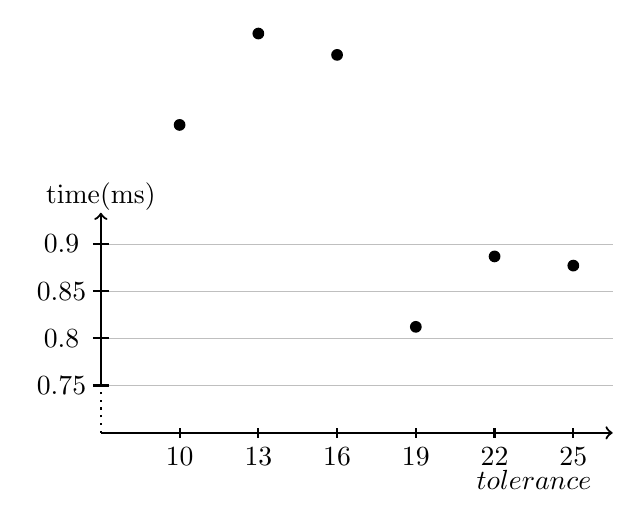
\begin{tikzpicture}[thick, yscale=12]
		%time axis
		\draw[->] (0,0.75) -- (0,0.933);
		\draw[dotted] (0, 0.7) -- (0,0.75);
		\node at (0, 0.95){time(ms)};
		
		\foreach \y in {0.75,0.8,0.85, 0.9}{
			\draw[very thin, lightgray] (0, \y)--(6.5, \y);
			\draw(-0.1, \y)--(0.1, \y);
			\node at (-0.5, \y){\y};
			
		}
		
		\draw[->] (0,0.7) -- (6.5, 0.7);
		\node at (5.5, 0.65){$tolerance$};
		\foreach \x in {0, 1, 2, ..., 5}{
			\draw(\x+1, 0.695)--(\x+1, 0.705);
		}
		\node at (1, 0.675){$10$};
		\node at (2, 0.675){$13$};
		\node at (3, 0.675){$16$};
		\node at (4, 0.675){$19$};
		\node at (5, 0.675){$22$};
		\node at (6, 0.675){$25$};
		\node at (1, 1.0259) [circle,fill,inner sep=1.5pt]{};
		\node at (2, 1.1226) [circle,fill,inner sep=1.5pt]{};
		\node at (3, 1.1) [circle,fill,inner sep=1.5pt]{};
		\node at (4, 0.8122) [circle,fill,inner sep=1.5pt]{};
		\node at (5, 0.8867) [circle,fill,inner sep=1.5pt]{};
		\node at (6, 0.8770) [circle,fill,inner sep=1.5pt]{};
%		\node at (1, 0.7607) [circle,fill,inner sep=1.5pt]{};
%		\node at (2, 0.7729) [circle,fill,inner sep=1.5pt]{};
%		\node at (3, 0.8121) [circle,fill,inner sep=1.5pt]{};
%		\node at (4, 0.8122) [circle,fill,inner sep=1.5pt]{};
%		\node at (5, 0.8867) [circle,fill,inner sep=1.5pt]{};
%		\node at (6, 0.8770) [circle,fill,inner sep=1.5pt]{};
		\end{tikzpicture}
		\centering
		\caption{Average run times of the\\ \textit{OutputSynchronizationConstraint} with 2\\ $response$ streams and a cluster distance of 2}
		\label{fig:OutputSynchronizationConstraintRuntime1}
	\end{minipage}\hfill
	\begin{minipage}{0.45\textwidth}
		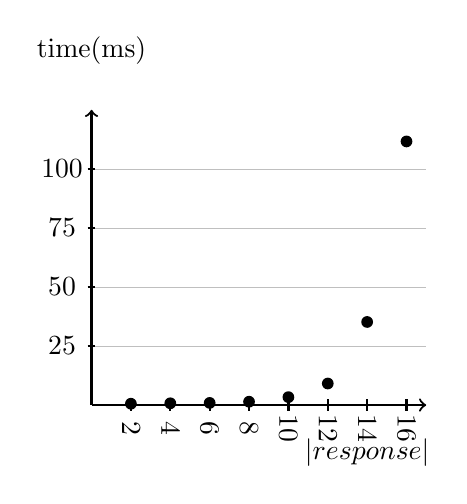
\begin{tikzpicture}[thick, yscale=0.03, xscale=0.5]
		%time axis
		\draw[->] (0,0) -- (0,125);
		\node at (0, 150){time(ms)};
		
		\foreach \y in {25, 50, 75, 100}{
			\draw[very thin, lightgray] (0, \y)--(8.5, \y);
			\draw(-0.1, \y)--(0.1, \y);
			\node at (-0.75, \y){\y};
			
		}
		
		\draw[->] (0,0) -- (8.5, 0);
		\node at (7, -20){$|response|$};
		\foreach \x in {0, 1, 2, ..., 7}{
			\draw(\x+1, 2.5)--(\x+1, -2.5);
		}
		\node[rotate=270] at (1, -10){$2$};
		\node[rotate=270] at (2, -10){$4$};
		\node[rotate=270] at (3, -10){$6$};
		\node[rotate=270] at (4, -10){$8$};
		\node[rotate=270] at (5, -10){$10$};
		\node[rotate=270] at (6, -10){$12$};
		\node[rotate=270] at (7, -10){$14$};
		\node[rotate=270] at (8, -10){$16$};
		\node at (1, 0.5628) [circle,fill,inner sep=1.5pt]{};
		\node at (2, 0.7489) [circle,fill,inner sep=1.5pt]{};
		\node at (3, 0.9039) [circle,fill,inner sep=1.5pt]{};
		\node at (4, 1.4093) [circle,fill,inner sep=1.5pt]{};
		\node at (5, 3.3479) [circle,fill,inner sep=1.5pt]{};
		\node at (6, 9.1158) [circle,fill,inner sep=1.5pt]{};
		\node at (7, 35.1766) [circle,fill,inner sep=1.5pt]{};
		\node at (8, 111.5996) [circle,fill,inner sep=1.5pt]{};
		\end{tikzpicture}
		\centering
		\caption{Average run times of the\\ \textit{OutputSynchronizationConstraint} with a cluster\\ distance of 16 and $tolerance=10$}
		\label{fig:OutputSynchronizationConstraintRuntime2}
	\end{minipage}\hfill
\end{figure}


\subsubsection{InputSynchronizationConstraint}
The traces for the evaluation of the \textit{InputSynchronizationConstraint} were generated with 2,3, 4 and 5 $stimulus$ streams, $tolerance$ values of 10 to 25 in steps of 3 and a distance between synchronization clusters of 2, 4, 8, 16 or 32. Similar to the previous constraint, traces with up to 202 $stimulus$ streams were tested in a second run.\\
Figure~\ref{fig:InputSynchronizationConstraintRuntime1} shows the run time of the monitor with the traces with three $stimulus$ streams and a fixed cluster distance of 2. The run times are nearly constant, which was expected by the analysis of the source code. Figure~\ref{fig:InputSynchronizationConstraintRuntime2} shows the average run time with a fixed cluster distance and $tolerance$ and an increasing number of $stimulus$ streams. As expected, the run times are increasing by the square of the number of $stimulus$ streams, but the increase is much larger than in the previous constraint.

\begin{figure}
	\centering
	\begin{minipage}{0.45\textwidth}
		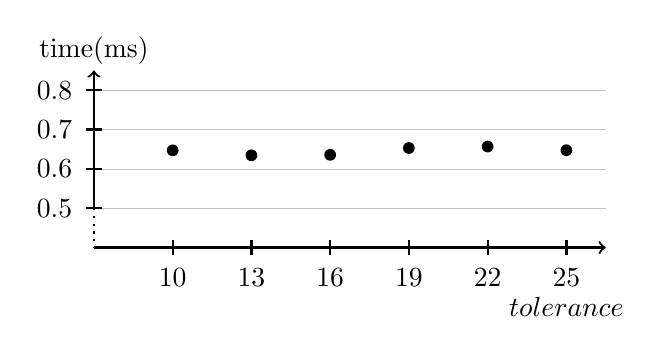
\begin{tikzpicture}[thick, yscale=5]
		%time axis
		\draw[->] (0,0.5) -- (0,0.85);
		\draw[dotted] (0, 0.5) -- (0,0.4);
		\node at (0, 0.9){time(ms)};
		
		\foreach \y in {0.5,0.6,0.7,0.8}{
			\draw[very thin, lightgray] (0, \y)--(6.5, \y);
			\draw(-0.1, \y)--(0.1, \y);
			\node at (-0.5, \y){\y};
			
		}
		%TODO neue Werte und Parameter
		\draw[->] (0,0.4) -- (6.5, 0.4);
		\node at (6, 0.25){$tolerance$};
		\foreach \x in {0, 1, 2, ..., 5}{
			\draw(\x+1, 0.38)--(\x+1, 0.42);
		}
		\node at (1, 0.325){$10$};
		\node at (2, 0.325){$13$};
		\node at (3, 0.325){$16$};
		\node at (4, 0.325){$19$};
		\node at (5, 0.325){$22$};
		\node at (6, 0.325){$25$};
		\node at (1, 0.647) [circle,fill,inner sep=1.5pt]{};
		\node at (2, 0.6344) [circle,fill,inner sep=1.5pt]{};
		\node at (3, 0.6356) [circle,fill,inner sep=1.5pt]{};
		\node at (4, 0.6529) [circle,fill,inner sep=1.5pt]{};
		\node at (5, 0.6566) [circle,fill,inner sep=1.5pt]{};
		\node at (6, 0.6473) [circle,fill,inner sep=1.5pt]{};
		\end{tikzpicture}
		\centering
		\caption{Average run times of the\\ \textit{InputSynchronizationConstraint} with 3\\ stimulus streams and a cluster distance of 2}
		\label{fig:InputSynchronizationConstraintRuntime1}
	\end{minipage}\hfill
		\begin{minipage}{0.45\textwidth}
			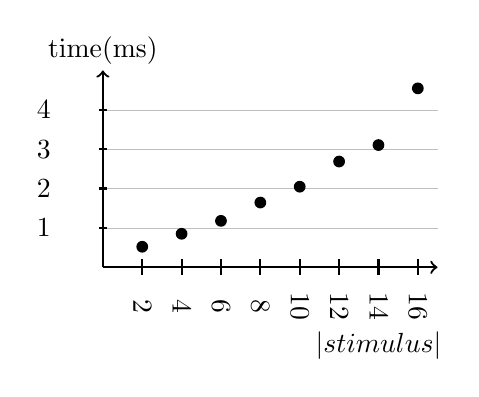
\begin{tikzpicture}[thick, yscale=0.5, xscale=0.5]
				%time axis
				\draw[->] (0,0) -- (0,5);
				\node at (0, 5.5){time(ms)};
				
				\foreach \y in {1, 2, 3, 4}{
					\draw[very thin, lightgray] (0, \y)--(8.5, \y);
					\draw(-0.1, \y)--(0.1, \y);
					\node at (-1.5, \y){\y};
					
				}
				
				\draw[->] (0,0) -- (8.5, 0);
				\node at (7, -2){$|stimulus|$};
				\foreach \x in {1,2,...,8}{
					\draw(\x, -0.2)--(\x, 0.2);
				}
				\node[rotate=270] at (1, -1){$2$};
				\node[rotate=270] at (2, -1){$4$};
				\node[rotate=270] at (3, -1){$6$};
				\node[rotate=270] at (4, -1){$8$};
				\node[rotate=270] at (5, -1){$10$};
				\node[rotate=270] at (6, -1){$12$};
				\node[rotate=270] at (7, -1){$14$};
				\node[rotate=270] at (8, -1){$16$};
				%*100
				\node at (1, 0.5213) [circle,fill,inner sep=1.5pt]{};
				\node at (2, 0.8505) [circle,fill,inner sep=1.5pt]{};
				\node at (3, 1.1792) [circle,fill,inner sep=1.5pt]{};
				\node at (4, 1.6437) [circle,fill,inner sep=1.5pt]{};
				\node at (5, 2.0464) [circle,fill,inner sep=1.5pt]{};
				\node at (6, 2.686) [circle,fill,inner sep=1.5pt]{};
				\node at (7, 3.1045) [circle,fill,inner sep=1.5pt]{};
				\node at (8, 4.5444) [circle,fill,inner sep=1.5pt]{};
			\end{tikzpicture}
			\centering
			\caption{Average run times of the\\ \textit{InputSynchronizationConstraint} with a cluster\\ distance of 2 and $tolerance=10$}
			\label{fig:InputSynchronizationConstraintRuntime2}
	\end{minipage}\hfill
\end{figure}

\subsubsection{EventChain}

The run times of the monitor for the correctness of event chains were also measured. The traces were generated with the same parameters as for the \textit{ReactionConstraint}. Figure~\ref{fig:EventChainRunTime1} and \ref{fig:EventChainRunTime2} show the results of this measurement, with fixed distances between subsequent $stimulus$ events of 1 and 128 timestamps and distances between $stimulus$ events and their associated $response$ event of 100, 200, ..., 1000. The run times in both cases are nearly constant, but the run times are slightly larger in figure~\ref{fig:EventChainRunTime1}. This is because the $stimulus$ and $response$ events occur in the same timestamps here, but not in figure~\ref{fig:EventChainRunTime2}.
\begin{figure}
		\begin{minipage}{0.45\textwidth}
		\centering
		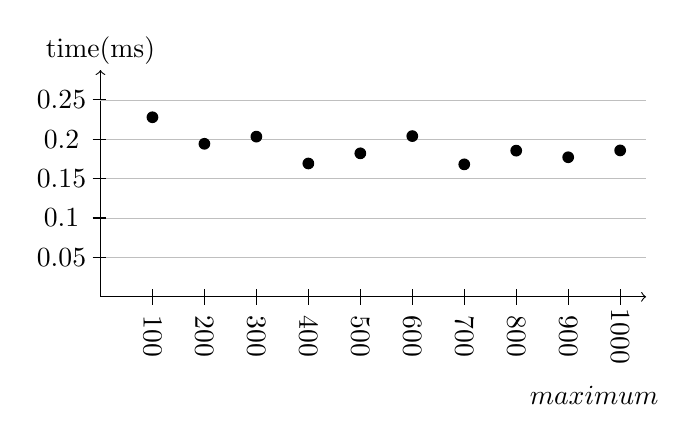
\begin{tikzpicture}[yscale=10, xscale=0.66]
			%time axis
			\draw[->] (0,0) -- (0,0.288);
			\node at (0, 0.3125){time(ms)};
			
			\foreach \y in {0.05, 0.1, 0.15, 0.2, 0.25}{
				\draw[very thin, lightgray] (0, \y)--(10.5, \y);
				\draw(-0.15, \y)--(0.1, \y);
				\node at (-0.75, \y){\y};
				
			}
			
			\draw[->] (0,0) -- (10.5, 0.0);
			\node at (9.5, -0.125){$maximum$};
			\foreach \x in {1, 2, ..., 9, 10}{
				\draw(\x, -0.01)--(\x, 0.01);
				\node[rotate=270] at (\x, -0.05){$\x00$};
			}
			\node at (1, 0.228) [circle,fill,inner sep=1.5pt]{};
			\node at (2, 0.1943) [circle,fill,inner sep=1.5pt]{};
			\node at (3, 0.2034) [circle,fill,inner sep=1.5pt]{};
			\node at (4, 0.1693) [circle,fill,inner sep=1.5pt]{};
			\node at (5, 0.1822) [circle,fill,inner sep=1.5pt]{};
			\node at (6, 0.2041) [circle,fill,inner sep=1.5pt]{};
			\node at (7, 0.1682) [circle,fill,inner sep=1.5pt]{};
			\node at (8, 0.1856) [circle,fill,inner sep=1.5pt]{};
			\node at (9, 0.1772) [circle,fill,inner sep=1.5pt]{};
			\node at (10, 0.1859) [circle,fill,inner sep=1.5pt]{};
		\end{tikzpicture}
		\centering
		\caption{Average run times of the\\\textit{EventChain} check with a distance between\\ subsequent $stimulus$ events of 1 and variable\\ $maximum$(\textit{ReactionConstraint} parameter)}
		\label{fig:EventChainRunTime1}
	\end{minipage}\hfill
	\begin{minipage}{0.45\textwidth}
	\centering
	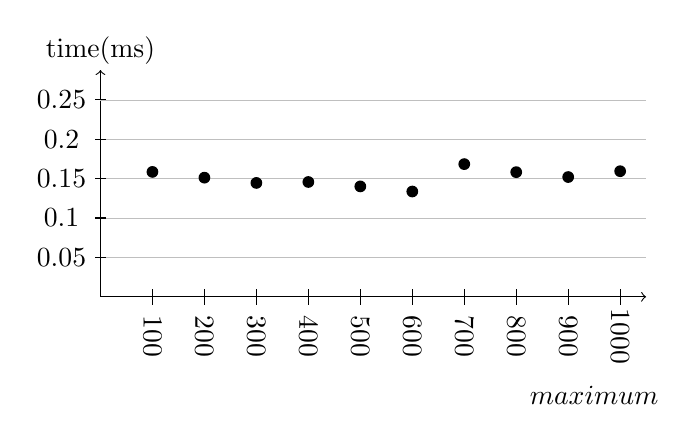
\begin{tikzpicture}[yscale=10, xscale=0.66]
	%time axis
		\draw[->] (0,0) -- (0,0.288);
		\node at (0, 0.3125){time(ms)};
		
		\foreach \y in {0.05, 0.1, 0.15, 0.2, 0.25}{
			\draw[very thin, lightgray] (0, \y)--(10.5, \y);
			\draw(-0.1, \y)--(0.1, \y);
			\node at (-0.75, \y){\y};
			
		}
		
		\draw[->] (0,0) -- (10.5, 0.0);
		\node at (9.5, -0.125){$maximum$};
		\foreach \x in {1, 2, ..., 9, 10}{
			\draw(\x, -0.01)--(\x, 0.01);
			\node[rotate=270] at (\x, -0.05){$\x00$};
		}
		\node at (1, 0.1586) [circle,fill,inner sep=1.5pt]{};
		\node at (2, 0.1513) [circle,fill,inner sep=1.5pt]{};
		\node at (3, 0.1446) [circle,fill,inner sep=1.5pt]{};
		\node at (4, 0.1458) [circle,fill,inner sep=1.5pt]{};
		\node at (5, 0.1402) [circle,fill,inner sep=1.5pt]{};
		\node at (6, 0.1337) [circle,fill,inner sep=1.5pt]{};
		\node at (7, 0.1685) [circle,fill,inner sep=1.5pt]{};
		\node at (8, 0.1583) [circle,fill,inner sep=1.5pt]{};
		\node at (9, 0.1521) [circle,fill,inner sep=1.5pt]{};
		\node at (10, 0.1595) [circle,fill,inner sep=1.5pt]{};
	\end{tikzpicture}
	\centering
	\caption{Average run times of the \\\textit{EventChain} check with a distance between\\ subsequent $stimulus$ events of 128 and variable\\ $maximum$(\textit{ReactionConstraint} parameter)}
	\label{fig:EventChainRunTime2}
\end{minipage}

\end{figure}

\subsection{Conclusion}
	%TODO Überleitung AUTOSAR ???
	The implementations offer the possibility to check if the timing constraints defined in TADL2 on input traces. As described in section~\ref{comparisonConstraints}, most of the AUTOSAR Timing Extensions can be described via the TADL2 Constraints, but semantic differences exist in some constraints. Most of these differences are further restrictions in the AUTOSAR definitions. For example, AUTOSARs \textit{BurstPatternEventTriggering} additionally defines the repetitions of bursts, while TADL2s \textit{BurstConstraint} does not specify them. As a result, the \textit{BurstPatternEventTriggering} can be monitored by the implementation of the \textit{BurstConstraint}, but not all violations can be found.\\
	Most of the implementations have acceptable run times. In the setting used for the run time measurement, the implementations of the  \textit{StrongDelay-}, \textit{Repeat-}, \textit{Repetition-}, \textit{ExecutionTime-}, \textit{Order-}, \textit{Sporadic-}, \textit{Periodic-}, \textit{Pattern-} and \textit{BurstConstraint} were processing more than one event per millisecond. It was shown that the constraint parameters of these constraints did not influence the run time. This was expected by the analysis of the source code, in which a constant run time of these implementations was predicted.\\
	The run times of the \textit{Delay-}, \textit{Arbitrary-}, \textit{Synchronization-} and the \textit{StrongSynchronization-}, \textit{Age-} and \textit{ReactionConstraint} are linear dependent on the constraint parameters and the run times per input timestamp was larger than one millisecond for certain constraint parameters and event constellations.\\
	The run times of the \textit{OutputSynchronization-} and \textit{InputsynchronizationConstraint} monitors are growing by the square of the number of input streams. While the average run times with a small number of input streams were below 1ms per input timestamp, it increased significantly when the number of input streams was increased. The run average run time per input timestamp of the \textit{OutputSynchronizationConstraint} with 16 $response$ streams was larger than 100ms.\\
	The run time for the check of the correctness of EventChains was constant at around 0.15ms per input event, therefore ca. 6600 events were processed per second. It must be noted that the memory usage of the \textit{OutputSynchronization-}, \textit{InputsynchronizationConstraint} and the check for the correctness of \textit{EventChains} is linear dependent on the number of events, which previously occurred in the streams. Consequently, the system's memory will be filled at some point when infinite long traces are observed, which means they cannot be monitored infinitely.\\
	
	
	
	
	%	In the measurement runs, the \textit{DelayConstraint} also had a constant run time below 1ms per Event, but in worst cases, the run time of the monitor can be linear dependent on one constraint parameter.\\
	%	The run time of the \textit{ArbitraryConstraint} is linear dependent on the length of the input parameters in all cases and increasing the length of the parameters by increases the run time by ca. 1 ms.\\
	%	The run time of the \textit{Synchronization-} and the \textit{StrongSynchronizationConstraint} is linear dependent on the number of input streams and the constraint parameter $tolerance$, while for the  \textit{SynchronizationConstraint} monitor, the linear growth by $tolerance$ is only reached in worst cases, in which the events do not occur in synchronization clusters.
	%
	%	
	%	The run times of the \textit{Age-} and \textit{ReactionConstraint} is linear dependent on the constraint parameter $maximum$. The implementation of the \textit{AgeConstraint} had average run time between 0.3ms and 15ms per timestamp with events, while the \textit{ReactionConstraint} had average run times between 0.3ms and 26ms.\\
 

